\documentclass[12pt, a4paper, oneside]{report}

% -------------------------------------------------
% Packages
% -------------------------------------------------
\usepackage[utf8]{inputenc}
\usepackage[T1]{fontenc}
\usepackage{lmodern}
\usepackage[english]{babel}

\usepackage{geometry}
\geometry{
    a4paper,
    left=3cm,
    right=2.5cm,
    top=3cm,
    bottom=3cm
}

\usepackage{setspace}
\onehalfspacing

\usepackage{graphicx}
\usepackage{float}
\usepackage{caption}
\usepackage{subcaption}
\usepackage{algorithmic}

\usepackage{amsmath, amssymb, amsthm}
\usepackage{booktabs}
\usepackage{array}
\usepackage{multirow}
\usepackage{longtable}

\usepackage{algorithm}
\usepackage{algpseudocode}

\usepackage{listings}
\usepackage{xcolor}

\usepackage{hyperref}
\hypersetup{
    colorlinks=true,
    linkcolor=blue,
    citecolor=blue,
    urlcolor=blue,
    pdftitle={Master Thesis},
    pdfauthor={Your Name}
}

% \usepackage[numbers]{natbib}

\usepackage{cite} 
% -------------------------------------------------
% Code listing style
% -------------------------------------------------
\lstdefinestyle{mystyle}{
    basicstyle=\ttfamily\small,
    breaklines=true,
    frame=single,
    numbers=left,
    numberstyle=\tiny,
    keywordstyle=\color{blue},
    commentstyle=\color{green!50!black},
    stringstyle=\color{red!70!black},
    showstringspaces=false
}
\lstset{style=mystyle}

% -------------------------------------------------
% Theorem environments
% -------------------------------------------------
\newtheorem{definition}{Definition}[chapter]
\newtheorem{theorem}{Theorem}[chapter]
\newtheorem{lemma}{Lemma}[chapter]

% -------------------------------------------------
% Thesis Information
% -------------------------------------------------
\newcommand{\thesistitle}{Uncertainty-Aware Bus ETA Prediction Under Drift with Segment-Level Risk Decomposition}
\newcommand{\thesisauthor}{Koray Düzgün - Mohammad Abdulsamad Abdulhakim}
\newcommand{\supervisor}{Tuwe Löfström}
\newcommand{\university}{Jönköping University}
\newcommand{\submissiondate}{05/2026}

% -------------------------------------------------
% Document
% -------------------------------------------------
\begin{document}

% -------------------------------------------------
% Title Page
% -------------------------------------------------
\begin{titlepage}
    \centering
    \vspace*{2cm}

    {\Huge \bfseries \thesistitle \par}
    \vspace{2cm}

    {\Large A Master's Thesis \par}
    \vspace{0.5cm}
    {\Large Master of Science in AI Engineering \par}

    \vspace{2cm}

    {\large by \par}
    \vspace{0.3cm}
    {\Large \bfseries \thesisauthor \par}
    \vfill

    \begin{flushleft}
        \textbf{Supervisor:} \supervisor \\
    \end{flushleft}

    \vfill

    {\large \department \par}
    {\large \faculty \par}
    {\large \university \par}
    \vspace{0.5cm}
    {\large \submissiondate \par}

\end{titlepage}

% -------------------------------------------------
% Front Matter
% -------------------------------------------------
\pagenumbering{arabic}


% ============================================================
% ABSTRACT
% ============================================================

\begin{abstract}

Bus arrival time predictions from machine learning models are often accurate on average but lack reliable uncertainty estimates. This thesis investigates conformal prediction as a distribution-free framework for producing prediction intervals around bus ETA estimates, evaluating its behaviour under temporal distribution shift and exploring strategies to improve interval efficiency and interpretability.

We use XGBoost models at both route and segment levels, wrapped with conformal prediction intervals via the calibrated\_explanations framework. Experiments are conducted on a real-world GTFS dataset from Astana, Kazakhstan, covering three bus routes over 55 days.

Three research questions are addressed. First, we measure the behaviour of static conformal prediction under temporal drift. Despite statistically significant distribution shift between calibration and test periods (Kolmogorov-Smirnov $p < 0.001$), static CP maintains marginal coverage close to the 90\% target (PICP = 0.875). The intervals are 66 minutes wide for trips that typically take 80--90 minutes. Given that marginal coverage is near the target but intervals are too wide for practical use, the second question becomes whether interval efficiency can be improved while keeping empirical coverage close to the nominal target. We evaluate online adaptive conformal methods and alternative nonconformity measures at the route level through a $4 \times 4$ factorial design of 16 configurations. Difficulty estimation reduces the Winkler Score by 11--14\% relative to the absolute baseline. Online recalibration reduces calibration error from 0.026 to 0.004. The best route-level configuration is Online Expanding $\times$ Mondrian + DE with Winkler Score 5,551, but it still produces intervals over 60 minutes wide. Third, we move beyond route-level optimisation and test segment-level uncertainty decomposition with route-level re-calibration. We predict each segment of the planned route at the moment of departure and exploit residual diversification during summation. This approach reduces interval width to 39 minutes with a Winkler Score of 4,035, a 37\% improvement over the static CP baseline (6,449) and a 27\% improvement over the best route-level configuration (5,551). Empirical coverage holds at 0.888 and uncertainty attribution identifies a small set of structural hotspots that account for the bulk of the per-trip uncertainty budget.

The results show that marginal coverage alone is a misleading indicator of CP quality because it hides interval inefficiency and conditional coverage variation across subgroups. Interval efficiency and spatial interpretability are the primary axes of improvement, and this thesis addresses both through adaptive nonconformity measures and segment-level decomposition.

\end{abstract}
\chapter{Introduction}

\section{Background}

Reliable travel time prediction is a core requirement for public transportation systems. When passengers and operators have access to accurate estimates of bus arrival times, scheduling improves, waiting times decrease, and trust in the transit service grows. For this reason, bus Estimated Time of Arrival (ETA) prediction has received sustained research attention over the past decade.

Machine learning methods have brought significant accuracy gains to this problem. Gradient boosting models such as XGBoost deliver strong performance on structured transit data with engineered temporal features \cite{Savithramma20241003}. Recurrent architectures including LSTM and GRU capture sequential dependencies in GPS trajectory data \cite{Munkhbayar2025695}. More recent work has introduced graph neural networks and Transformer-based models to represent spatial relationships between route segments \cite{Lin202330384, Ma2022}. Hybrid frameworks that combine multiple paradigms have further pushed prediction accuracy \cite{Wang2018858, Chu202376095}.

However, most ETA models produce only a single point estimate. They optimise for average error metrics such as MAE or RMSE and do not indicate how confident the prediction is. In practice, however, the reliability of a prediction matters as much as its accuracy. A passenger benefits more from knowing that a bus will arrive between 12:05 and 12:15 with 90\% confidence than from a single estimate of 12:10 with no indication of how trustworthy that number is.

This gap between prediction accuracy and prediction reliability becomes especially problematic under non-stationary conditions. Bus travel times are influenced by traffic congestion, weather, passenger demand, and operational disruptions. These factors change over time, causing the statistical properties of travel time distributions to shift. A model trained and calibrated on one period may produce poorly calibrated uncertainty estimates when deployed in a later period. This phenomenon, known as temporal distribution shift or concept drift, has been documented as a major challenge in transportation forecasting \cite{Du2021402, Han20234100}.

Existing approaches to uncertainty estimation, including Bayesian methods and Kalman filtering, face limitations in scalability or distributional assumptions that reduce their applicability to bus operations (reviewed in Chapter~2). Conformal prediction offers a distribution-free alternative that produces prediction intervals with finite-sample coverage guarantees and can wrap around any point prediction model \cite{Lei20181094}. Recent work has extended conformal methods to handle temporal dependence \cite{Chernozhukov2018732, Xu202111559} and non-stationarity \cite{Zaffran202225834, Gibbs2024, Barber2023816}. However, the application of conformal prediction to bus ETA under temporal drift has received little empirical investigation.

\section{Problem Statement and Research Gap}

The literature on bus ETA prediction shows three specific gaps that this thesis addresses.

First, conformal prediction has been studied primarily in general machine learning settings. A small number of studies have applied it to transportation forecasting \cite{Petelin2024}, but we found limited empirical evidence on how coverage degrades over time due to temporal distribution shift in bus ETA specifically. The exchangeability assumption that conformal prediction relies on is known to break under drift, yet quantitative evidence for how this affects coverage in the bus domain is scarce.

Second, online and adaptive conformal methods have been proposed in the methodological literature \cite{Zaffran202225834, Gibbs2024, Angelopoulos2023}, but they have not been compared against static conformal prediction in a controlled bus ETA setting. It is not known whether sequential calibration updates can reduce calibration error, which window strategy is most effective, or whether alternative nonconformity measures such as Mondrian binning and difficulty-based normalisation provide additional efficiency benefits.

Third, segment-level modelling has been shown to improve point prediction accuracy by capturing local traffic dynamics \cite{Chen201160, Dunne2023141}. However, the question of how to decompose prediction uncertainty across segments while keeping the route-level calibration valid has not been addressed. The literature contains link-based and section-based prediction models, but not a framework that attributes route-level prediction uncertainty to specific spatial components in a statistically grounded way.

\section{Purpose and Research Questions}

The purpose of this thesis is to investigate the reliability of conformal prediction for bus travel time uncertainty estimation under temporal distribution shift, and to evaluate strategies for improving interval efficiency and interpretability.

The study is guided by three research questions:

\begin{enumerate}
    \item[\textbf{RQ1:}] How does temporal distribution shift affect the empirical coverage and interval efficiency of conformal prediction for bus ETA?

    \item[\textbf{RQ2:}] To what extent can adaptive conformal prediction methods reduce calibration error and improve interval efficiency compared to static conformal prediction under temporal drift?

    \item[\textbf{RQ3:}] Can segment-level decomposition improve interval efficiency and support interpretable uncertainty attribution, and what is the resulting effect on empirical coverage?
\end{enumerate}

\chapter{Literature Review}

This chapter reviews the literature relevant to this thesis. It covers five areas: point prediction methods for bus ETA, uncertainty estimation in transportation, conformal prediction as a distribution-free alternative, approaches to handling temporal drift, and segment-level decomposition for interpretability. Each section identifies the state of the art and its limitations, leading to the gaps that this thesis addresses.

\section{Point Prediction for Bus ETA}

Bus arrival time prediction has progressed from statistical methods to machine learning and deep learning. Recurrent neural networks, especially LSTM and GRU architectures, have become standard tools for modelling temporal dependencies in GPS trajectory data \cite{Munkhbayar2025695}. Hybrid approaches that combine deep learning with filtering techniques, such as particle filters, allow predictions to adapt to changing traffic conditions \cite{An202288}. Graph-based models and Transformer architectures capture spatial relationships between route segments and have improved accuracy further \cite{Sun20201820, Lin202330384, Ma2022}.

Tree-based ensemble methods remain competitive. XGBoost, in particular, performs well on structured tabular data when temporal features are carefully engineered \cite{Savithramma20241003}. Hybrid frameworks that combine linear, deep, and recurrent components have also been proposed to capture both memorization and generalization patterns \cite{Wang2018858, Chu202376095}.

Data quality is a recurring concern. Preprocessing and feature engineering strongly affect prediction performance \cite{Reich20202843}. Some studies incorporate auxiliary information, such as driver behaviour \cite{Sun20224037} or external traffic forecasts \cite{Tran20202957}, to enrich the feature space.

The vast majority of ETA models still produce deterministic point predictions. They optimise for average error metrics and do not indicate how confident the prediction is. This is a fundamental limitation for operational settings where the reliability of a prediction matters as much as its accuracy. These advances in point prediction accuracy therefore motivate the need for reliable uncertainty quantification: a well-calibrated interval is only as useful as the point predictor it wraps.

\section{Uncertainty Estimation in Transportation}

Point predictions alone are insufficient for operational transit systems. A line of research has therefore explored probabilistic forecasting for bus travel time. Bayesian methods provide a principled framework for this. A Bayesian Gaussian Mixture Model has been proposed to capture multimodal traffic behaviour and produce full predictive distributions \cite{Chen20231516}. In this approach, Markov Chain Monte Carlo (MCMC) inference is used to approximate the posterior distribution of the model parameters, allowing the method to represent uncertainty beyond a single point estimate. Functional Data Analysis and Bayesian Support Vector Regression have also been compared for bus arrival time reliability analysis, showing the benefit of connecting prediction with reliability assessment \cite{Huang2021}.

However, Bayesian approaches are computationally expensive. MCMC sampling does not scale well to large networks or real-time settings. Bayesian models also require distributional assumptions that may not hold in complex urban environments.

Quantile-based and interval-based methods are more practical. They estimate conditional quantiles or prediction intervals directly, without fitting a full posterior distribution. Uncertainty quantification in deep spatio-temporal forecasting has been examined, arguing that predictive performance should be evaluated by calibration and reliability, not just accuracy \cite{Wu20211841}. Bus travel time prediction has also been framed as conditional density estimation, enabling the computation of delay probabilities and service-level risk measures \cite{Ricard2022}. Related work on travel demand \cite{Peng2025} and passenger flow prediction \cite{Mu2025118} shows a broader trend toward quantifying uncertainty in transportation systems.

The evaluation of uncertainty has also received attention. Metrics such as Prediction Interval Coverage Probability (PICP), interval width, and Continuous Ranked Probability Score (CRPS) are increasingly used alongside traditional error metrics to assess whether uncertainty estimates are reliable \cite{Wu20211841, Zhang2024139789}.

A common limitation across these approaches is the lack of robustness under temporal distribution shift. When traffic patterns change over time, uncertainty estimates calibrated on historical data may become unreliable even when point predictions remain acceptable. Bayesian and quantile-based methods also require distributional assumptions or significant computational resources that limit their applicability in real-time transit settings, motivating the distribution-free conformal approach adopted in this thesis.

\section{Conformal Prediction}

Conformal prediction addresses many of the limitations above. It is a distribution-free framework that produces prediction intervals with finite-sample coverage guarantees, without assuming any particular error distribution. It is model-agnostic and can wrap around any point predictor.

Distribution-free predictive inference for regression has been formalized, establishing split conformal prediction as a general-purpose tool \cite{Lei20181094}. Conformalized Quantile Regression (CQR) combines quantile regression with conformal calibration to produce adaptive intervals in heteroskedastic settings \cite{Romano2019}. This is relevant for bus ETA, where prediction difficulty varies across trips.

One challenge for applying conformal prediction to transportation data is temporal dependence. Classical conformal methods assume exchangeability between calibration and test data. Conformal inference for dependent data has been studied \cite{Chernozhukov2018732}, and conformal intervals for dynamic time series have been proposed \cite{Xu202111559}. These works lay the theoretical groundwork for time-series applications.

Theoretical foundations for prediction beyond the exchangeability assumption have been studied by Barber et al.~\cite{Barber2023816}. More specialized extensions of conformal methods include multi-horizon forecasting \cite{Lopes2024345}, covariate shift handling \cite{Jonkers2024406}, and kernel-based weighted methods \cite{Lee202565354}.

Direct application of conformal prediction to transportation remains limited. Conformalized quantile regression has been applied to traffic forecasting and shown to produce calibrated intervals in this domain \cite{Petelin2024}. However, the behaviour of conformal prediction under temporal drift in bus ETA has not been empirically studied.

The variants of CP differ in which assumptions they require. Classical split CP requires exchangeability between calibration and test data. CQR~\cite{Romano2019} preserves this assumption while adapting interval width through an underlying quantile regression model. Mondrian CP~\cite{vovk2003mondrian} maintains the finite-sample guarantee within each bin, provided exchangeability holds within those bins. Difficulty-normalised CP adapts interval width to sample difficulty without changing the coverage guarantee under exchangeability. The route-level re-calibration proposed in this thesis (Experiment~3) is a variant of split CP applied to route-level aggregates of segment predictions; it inherits the guarantee under exchangeability but is applied in the same empirically evaluated, non-exchangeable temporal setting as the other methods.

These extensions demonstrate that conformal prediction can be adapted for time-series settings, but none have been evaluated on real GTFS bus data under measured temporal drift --- a gap this thesis addresses empirically.

\section{Temporal Distribution Shift and Concept Drift}

Traffic conditions are inherently non-stationary. Travel time distributions shift due to time-of-day effects, seasonal trends, weather, incidents, and infrastructure changes. This causes a mismatch between the data a model was trained on and the data it encounters during deployment.

Several adaptive learning approaches have been proposed. AdaRNN adjusts its internal representations across changing domains by identifying which temporal patterns are stable and which are shifting \cite{Du2021402}. A proactive drift detection framework has been proposed that anticipates distributional changes before errors accumulate \cite{Zhao20252020}. A two-stage meta-learning approach separates longer-term trends from short-term deviations, which fits the mixed nature of drift in transportation \cite{Chen20254869}.

Within transportation, online learning has been shown to outperform static models for traffic congestion prediction \cite{Manibardo2020}. For bus ETA specifically, the iETA framework updates predictions incrementally as new data arrives, avoiding full retraining while managing the balance between plasticity and stability \cite{Han20234100}. Incremental clustering for non-stationary traffic representations has also been proposed \cite{Tsai20223237}.

Most of these methods focus on maintaining point prediction accuracy under drift. Less attention has been given to whether uncertainty estimates remain reliable when the underlying distribution changes. A model can maintain acceptable average error while producing badly miscalibrated confidence intervals during transition periods.

On the uncertainty side, Adaptive Conformal Inference (ACI) \cite{Zaffran202225834} is an online learning procedure that adjusts the significance level at each time step based on whether the previous prediction was covered. ACI is not a conformal method itself; it is a sequential update rule that modifies the target level fed into any underlying interval construction procedure. Its guarantee is on long-run average coverage rather than finite-sample coverage. Gibbs and Cand\`es \cite{Gibbs2024} extended this idea to arbitrary distribution shifts, and Angelopoulos et al.~\cite{Angelopoulos2023} connected interval adjustment with PID control for time series. These methods represent a bridge between drift adaptation and uncertainty estimation, though they have not been evaluated in the bus ETA domain. Collectively, the drift literature focuses on maintaining point prediction accuracy; whether uncertainty estimates remain reliable under the same conditions is the central empirical question of this thesis.

\section{Segment-Level Decomposition and Interpretability}

Route-level ETA prediction treats the entire trip as one target, hiding the local structure that generates the total travel time. Segment-level decomposition addresses this by predicting travel time for individual stop-to-stop segments and aggregating the results.

Link-based and section-based models have been compared, showing that finer spatial decomposition captures local variability better \cite{Chen201160}. Segment-based prediction has been confirmed to outperform whole-route prediction by allowing each part of the route to respond to its own conditions \cite{Dunne2023141}. Separating running time from dwell time at the segment level further improves interpretability \cite{Baptista20121620}.

A known challenge is error accumulation. When segments are predicted independently and summed, errors can compound along the route. Modeling conditional dependencies between adjacent segments has been shown to address this problem \cite{Buchel2022}. Route-level distributions can also be synthesized from segment distributions \cite{Isukapati201371, Eisele2015286}.

Real-time traffic information is particularly useful at the segment level, since congestion and signal delays act locally \cite{Ma2019536, Julio2016250}. Graph neural networks provide tools for modelling spatial structure between segments \cite{Ma2022, Zhang202115008}. Explainability-oriented modelling has also been applied to make segment-level ETA predictions more transparent \cite{Warnakulasuriya20242131}.

Most segment-level studies still focus on point prediction accuracy. The question of how to decompose prediction uncertainty across segments, while keeping the route-level calibration valid, has not been addressed. The literature shows how to predict local travel times better, but not how route-level uncertainty can be attributed to specific spatial components in a statistically grounded way. These studies establish the value of segment-level modelling for accuracy, but do not address how route-level uncertainty should be calibrated after segment-level aggregation --- the problem Experiment~3 investigates.

\chapter{Methodology}
\label{ch:methodology}



% ============================================================
\section{Research Design}
\label{sec:research_design}
% ============================================================

This study employs a quantitative experimental research design to investigate the reliability of conformal prediction for bus travel time uncertainty estimation under temporal distribution shift. The research follows a systematic pipeline consisting of six stages: data acquisition and exploration, preprocessing and cleaning, feature engineering, baseline point prediction with XGBoost, conformal prediction for uncertainty quantification, and segment-level uncertainty decomposition.

\subsection{Research Framework Overview}
\label{subsec:framework_overview}

Figure~\ref{fig:framework_overview} presents the overall research framework. The pipeline begins with raw bus GPS trajectories and proceeds through preprocessing, feature engineering, and model training. The trained XGBoost model generates point predictions, which are then wrapped with conformal prediction to produce prediction intervals with nominal coverage guarantees under exchangeability. Finally, segment-level decomposition attributes route-level uncertainty to individual route segments.

\begin{figure}[H]
    \centering
    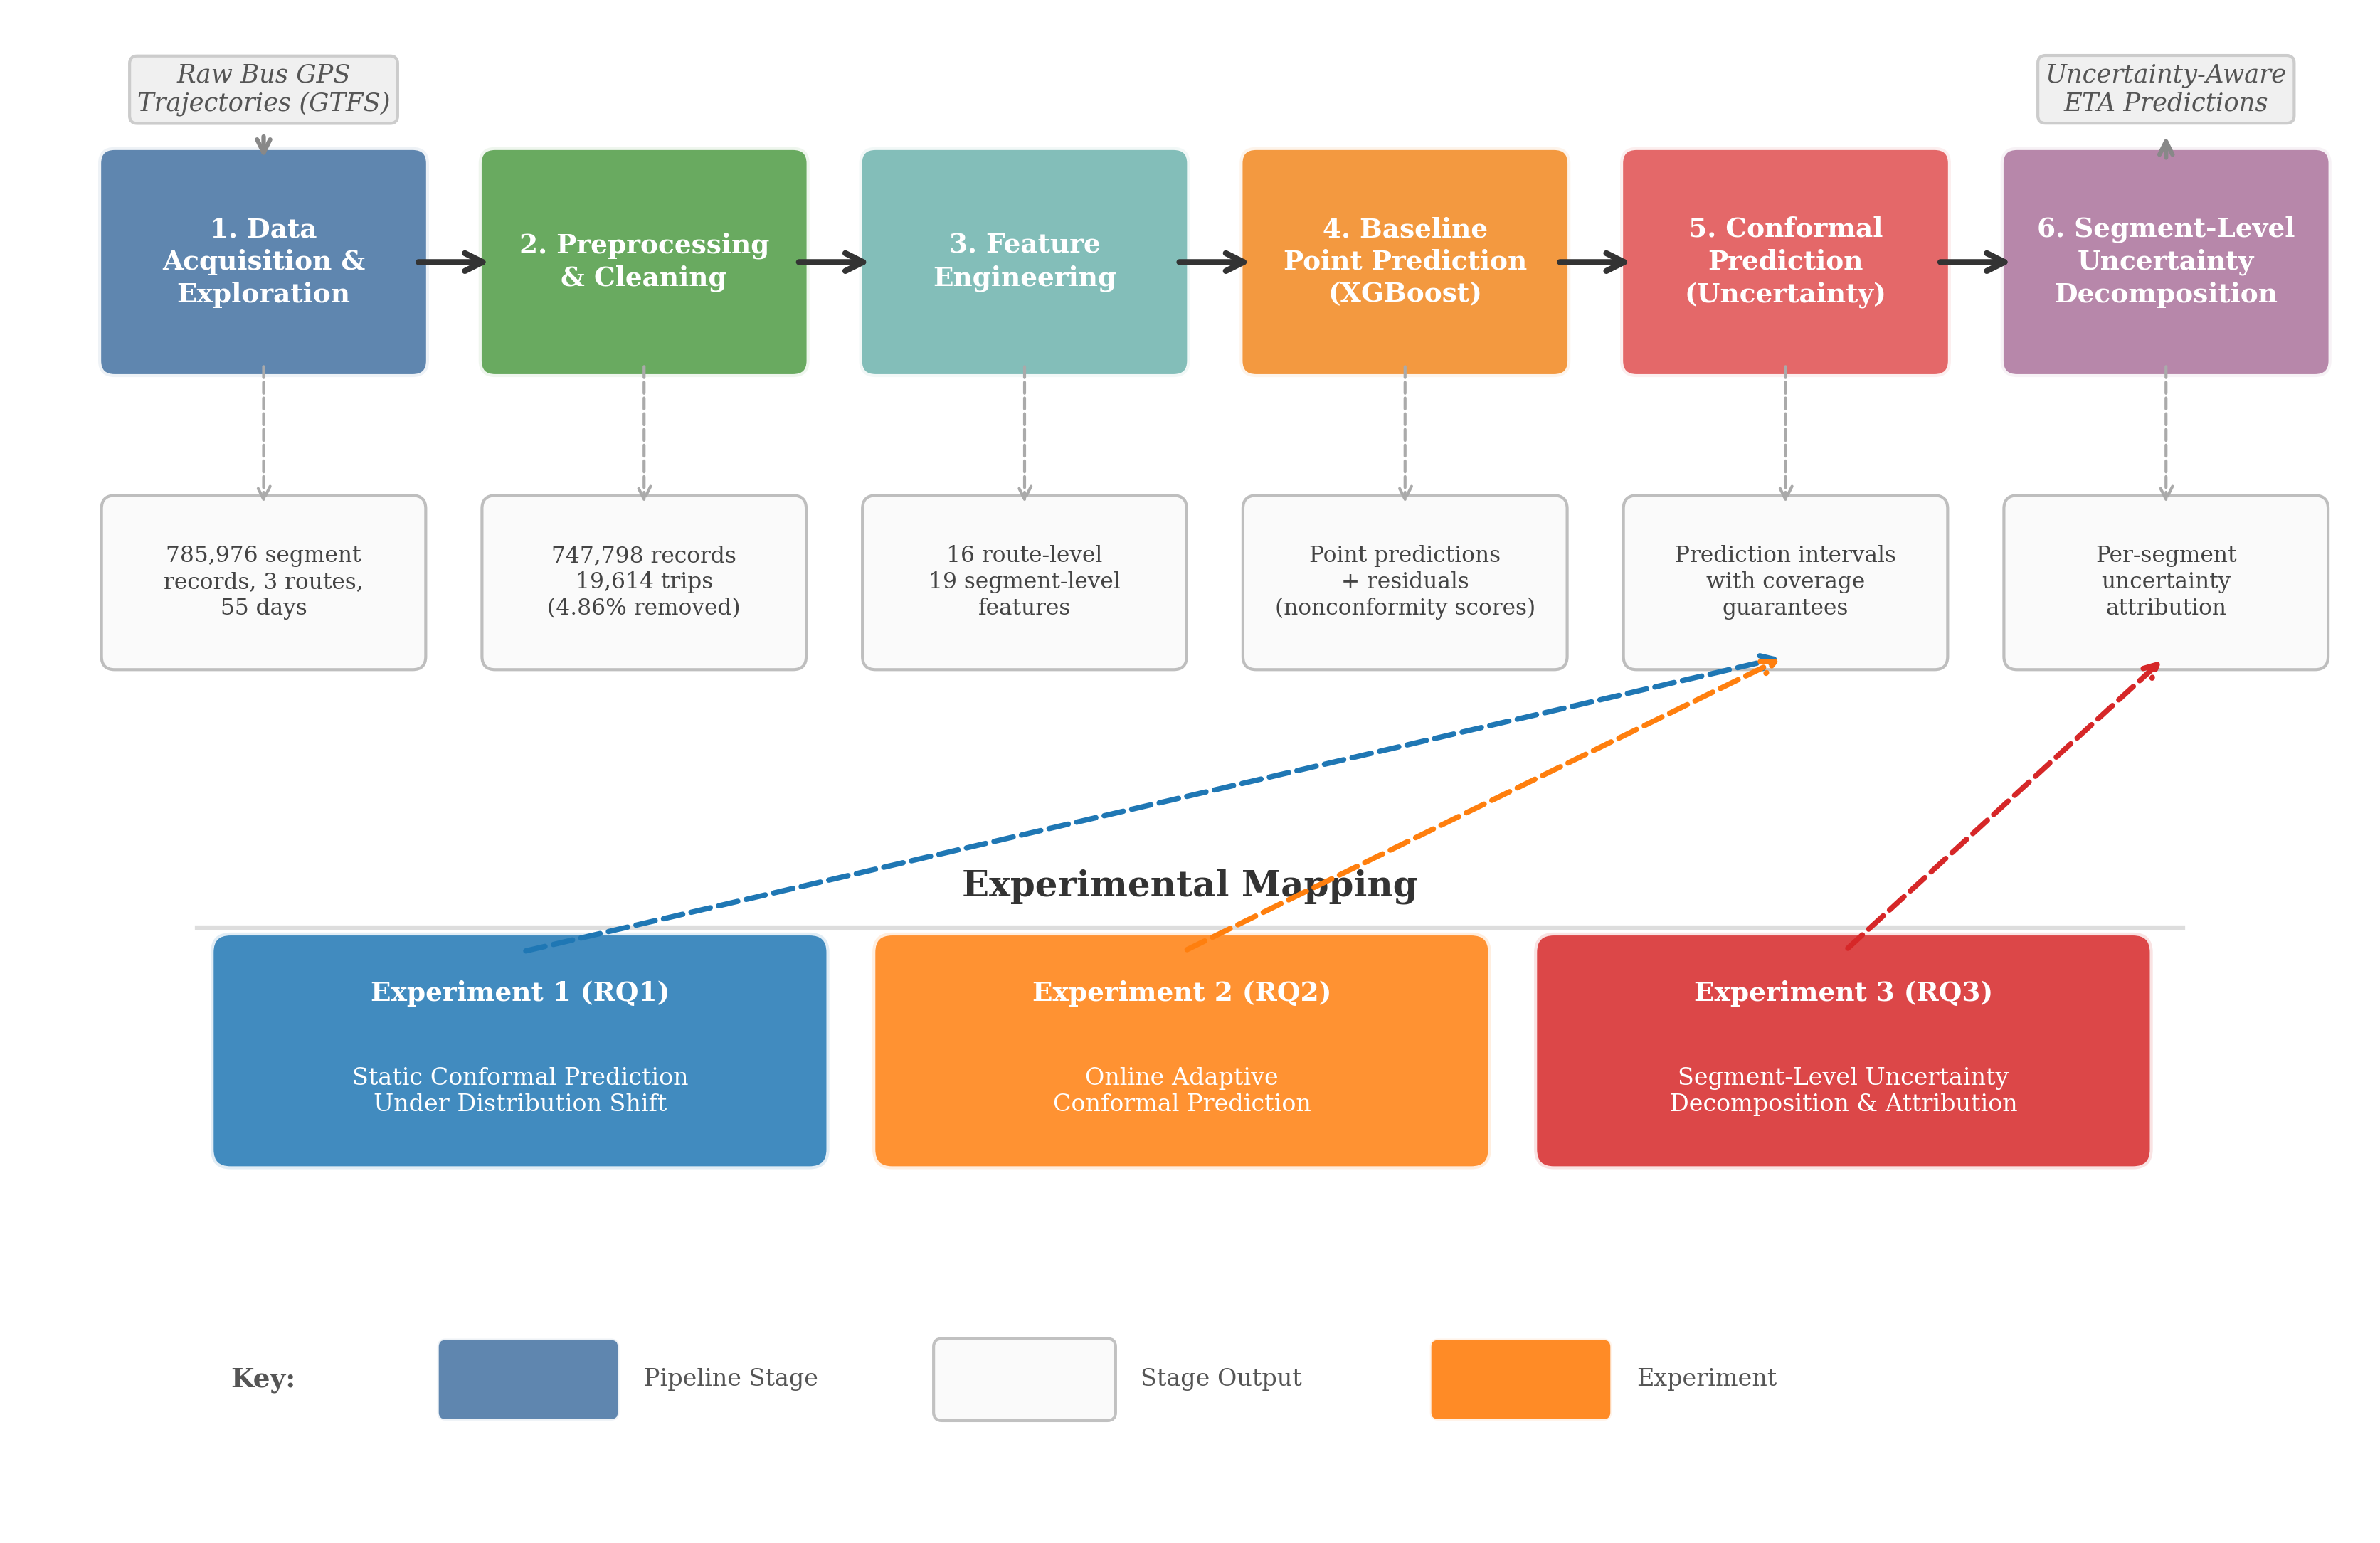
\includegraphics[width=\textwidth]{figures/3_1.png}
    \caption{End-to-end research framework. Raw bus GPS trajectories are preprocessed and enriched with engineered features. An XGBoost model generates point predictions, which are then wrapped with conformal prediction to produce prediction intervals. Segment-level decomposition attributes route-level uncertainty to individual route segments.}
    \label{fig:framework_overview}
\end{figure}

Each stage feeds into the next. Experiment~1 (RQ1) evaluates static conformal prediction under temporal distribution shift. Experiment~2 (RQ2) compares online adaptive conformal methods against the static baseline, including alternative adaptive calibration strategies such as Mondrian binning and difficulty-based normalisation. Experiment~3 (RQ3) investigates segment-level uncertainty decomposition for interpretable spatial risk attribution, evaluating the resulting efficiency--coverage trade-off.

\subsection{Temporal Split Strategy}
\label{subsec:temporal_split}

To simulate temporal distribution shift, the dataset is divided into weekly blocks assigned to specific roles. Table~\ref{tab:temporal_split} shows the split strategy.

\begin{table}[H]
\centering
\caption{Temporal split strategy for training, calibration, and evaluation.}
\label{tab:temporal_split}
\begin{tabular}{llrl}
\toprule
\textbf{Period} & \textbf{Weeks} & \textbf{Trips} & \textbf{Purpose} \\
\midrule
Training & W1--W3 (Jul~29 -- Aug~18) & 7,619 & XGBoost model training \\
Calibration & W4 (Aug~19 -- Aug~25) & 2,745 & CP calibration set \\
Test-Near & W5 (Aug~26 -- Sep~1) & 2,726 & Minimal drift evaluation \\
Test-Mid & W6 (Sep~2 -- Sep~8)$^\dagger$ & 1,844 & Moderate drift evaluation \\
Test-Far & W7--W8 (Sep~9 -- Sep~21) & 4,751 & Maximum drift evaluation \\
\bottomrule
\multicolumn{4}{l}{\footnotesize $^\dagger$ Excludes anomalous dates Sep~3--4 (5 usable days).}
\end{tabular}
\end{table}

September 3 and 4 were excluded from the analysis because their record counts (3,146 and 111, respectively) fall far below the daily norm of 10,000 to 18,000. The drop occurred simultaneously across all three routes, indicating a system-wide data collection failure rather than a route-specific service disruption. Including these dates would introduce artificial sparsity into the W6 test period and distort the coverage and interval width measurements. A threshold of 5,000 records per day was applied to identify and remove such dates, reducing the observation period from 55 to 53 usable days.

The three-level test period design (Near, Mid, Far) creates a temporal gradient for measuring coverage degradation under distribution shift. Test-Near is temporally closest to the calibration period and should exhibit minimal drift, while Test-Far is 2--4 weeks away and represents the most challenging evaluation condition.

\begin{figure}[H]
    \centering
    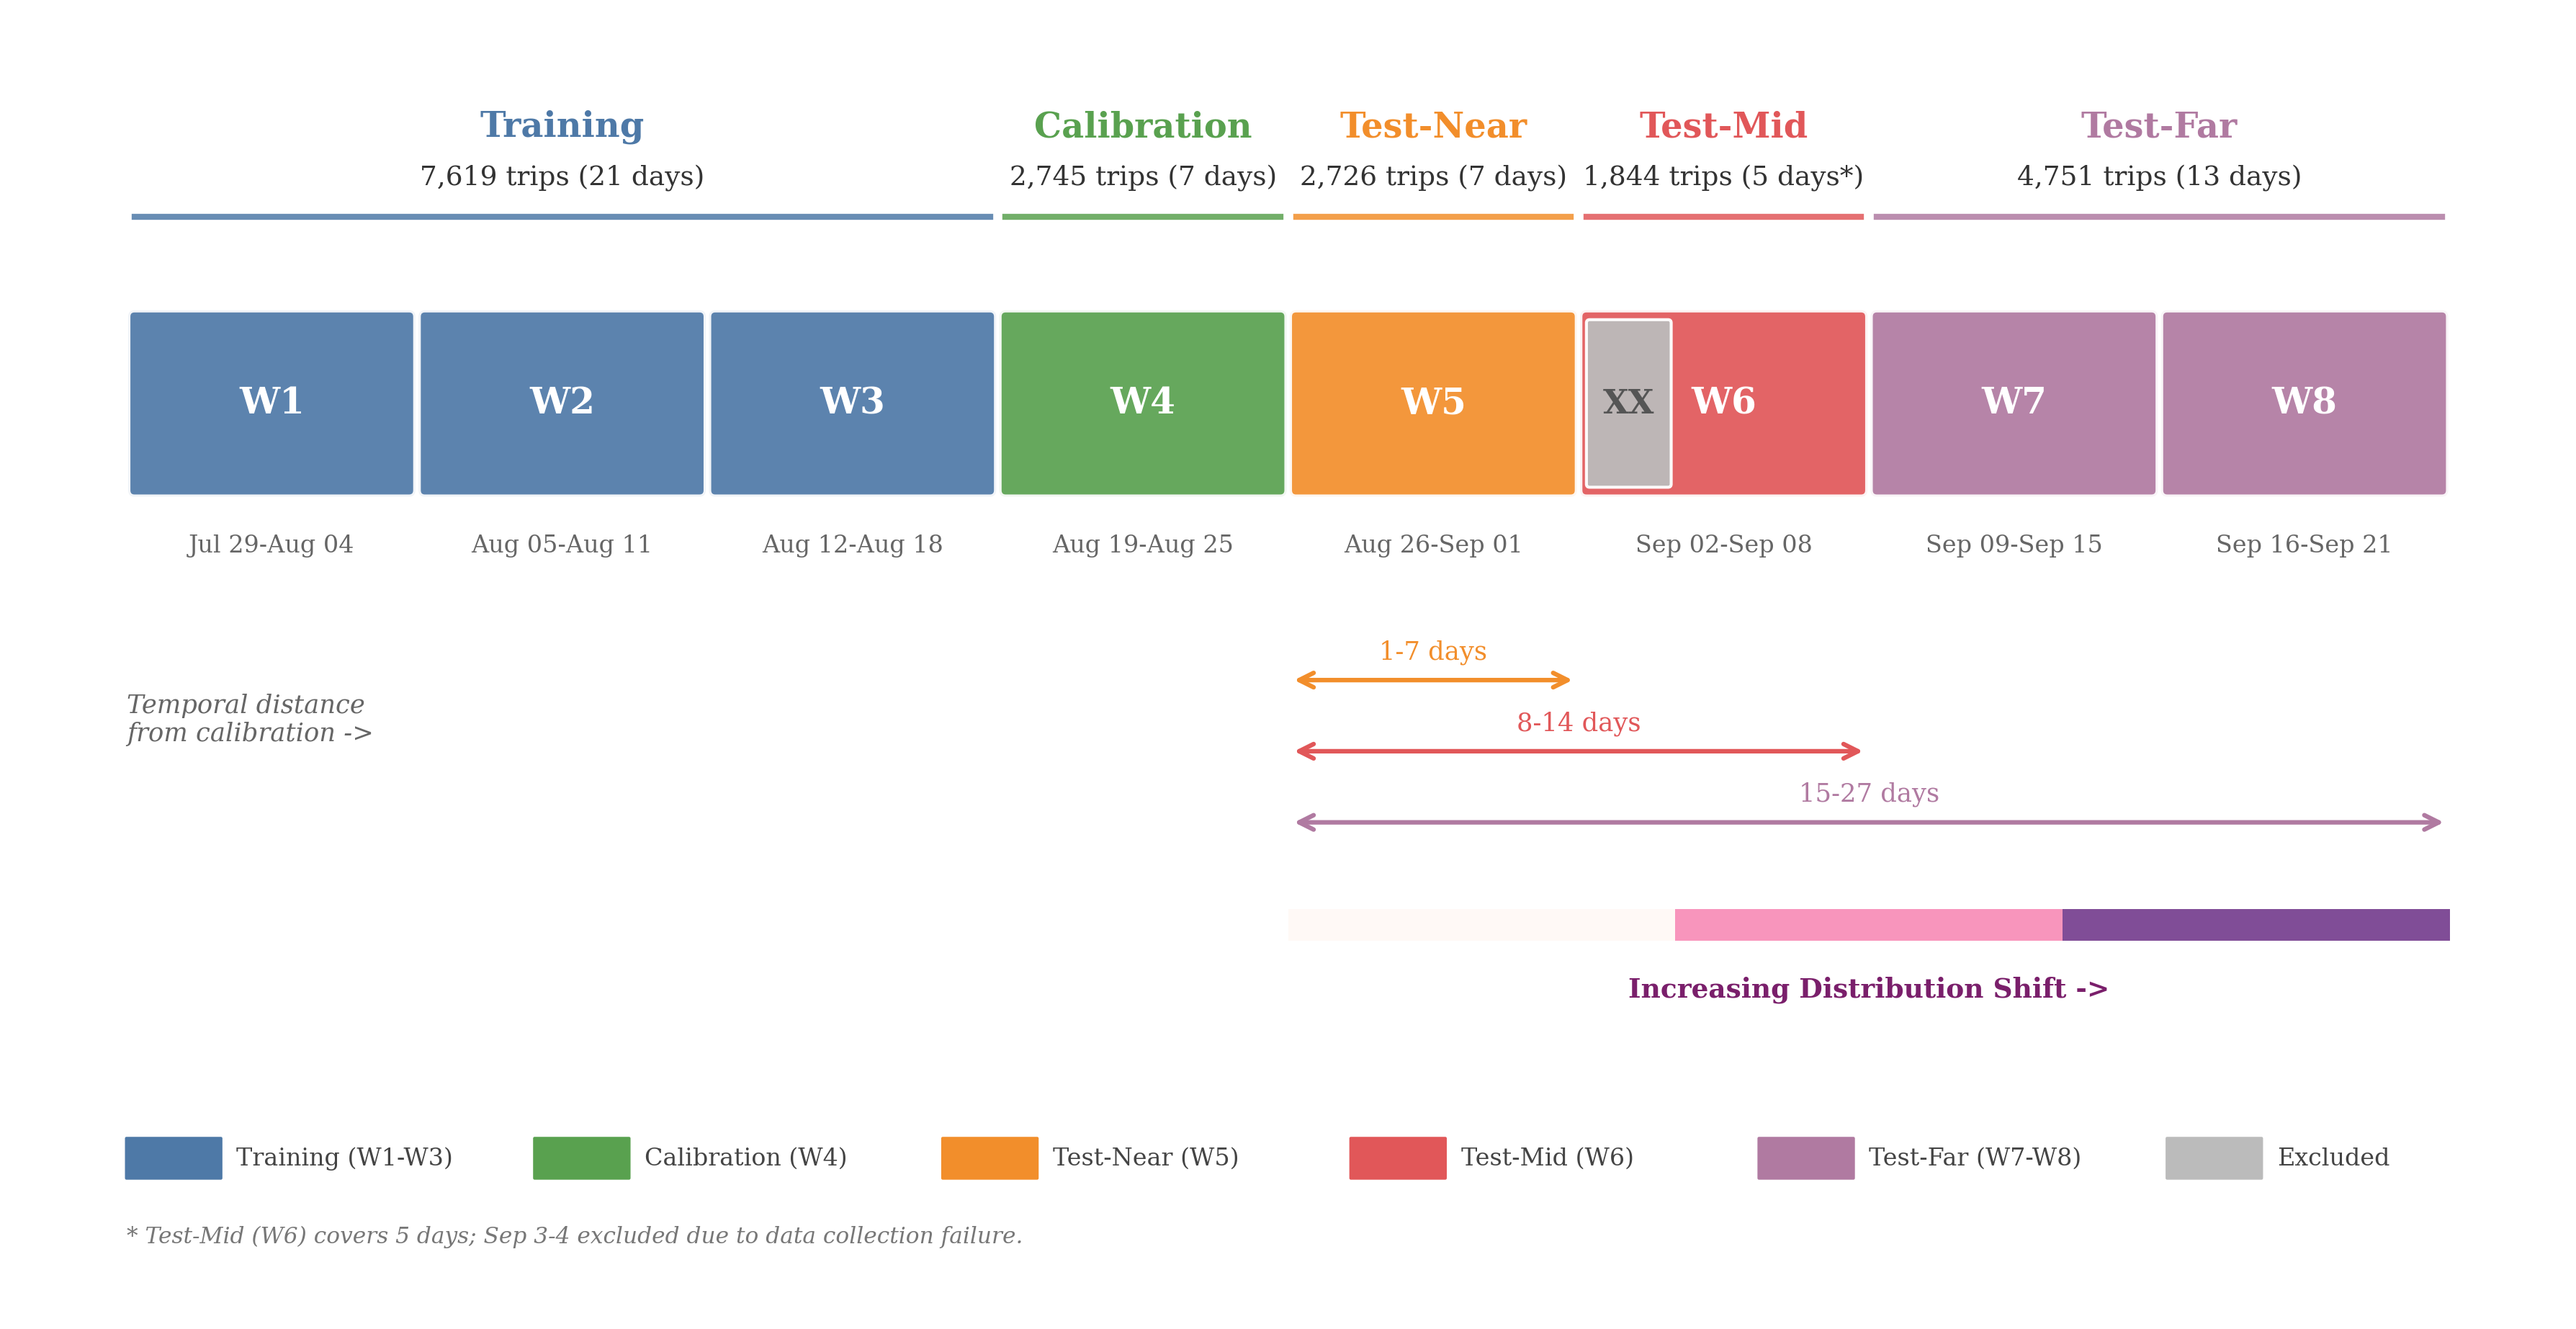
\includegraphics[width=\textwidth]{figures/3_2.png}
    \caption{Temporal split of the 55-day dataset into training (W1--W3), calibration (W4), and three test periods of increasing temporal distance. This design enables systematic evaluation of coverage degradation under distribution shift.}
    \label{fig:temporal_split}
\end{figure}

\subsection{Experimental Design}
\label{subsec:experimental_design}

Table~\ref{tab:experimental_matrix} summarizes the three experiments and their relationship to the research questions.

\begin{table}[H]
\centering
\caption{Summary of the three experiments.}
\label{tab:experimental_matrix}
\begin{tabular}{llll}
\toprule
& \textbf{Experiment~1} & \textbf{Experiment~2} & \textbf{Experiment~3} \\
\midrule
\textbf{Research Q.} & RQ1 & RQ2 & RQ3 \\
\textbf{Focus} & Coverage under drift & Adaptive calibration & Spatial decomposition \\
\textbf{Model level} & Route & Route & Segment $\rightarrow$ Route \\
\textbf{CP type} & Static & Online + alternatives & Normalised + re-calibration \\
\textbf{Key metric} & PICP degradation & Coverage improvement & Attribution + calibration \\
\textbf{Baseline} & Nominal 90\% & Static CP (Exp.~1) & Direct route CP \\
\bottomrule
\end{tabular}
\end{table}

\subsection{Methodological Choices and Alternatives}
\label{subsec:methodological_choices}

Several design choices in this study merit brief justification, as alternatives were available.

\textbf{XGBoost over deep learning models.} LSTM, GRU, and Transformer architectures have shown strong performance on bus ETA data. However, they require sequence-level data preprocessing and longer training cycles. Since the primary goal of this thesis is to evaluate uncertainty quantification strategies rather than to push point prediction accuracy, XGBoost provides a computationally tractable baseline that supports the extensive conformal calibration experiments without introducing model-specific complications orthogonal to the research questions.

\textbf{Split conformal prediction over Bayesian methods.} Bayesian approaches provide full predictive distributions but require distributional assumptions and scale poorly to large datasets with real-time requirements. Split CP makes no assumptions about the error distribution, wraps any pre-trained model, and requires only a one-time calibration pass. This aligns with the study's goal of evaluating a practically deployable uncertainty framework.

\textbf{Split CP over Conformalized Quantile Regression.} CQR~\cite{Romano2019} can produce tighter intervals in heteroskedastic settings by using a quantile regression model. However, it requires training and tuning an additional quantile regression layer on top of the point predictor, adding complexity. Since this thesis evaluates calibration behaviour and efficiency across multiple NCM variants, split CP provides a cleaner baseline that isolates the contribution of each component.

\textbf{No model retraining in online experiments.} The XGBoost model is kept fixed across all experiments while only the calibration set is updated (Experiment~2). This isolates the contribution of conformal recalibration from the contribution of model retraining, providing a cleaner answer to RQ2. In a real deployment, periodic retraining would complement online recalibration.

% ============================================================
\section{Data Collection}
\label{sec:data_collection}
% ============================================================

% ------------------------------------------------------------
\subsection{Dataset}
\label{subsec:dataset}
% ------------------------------------------------------------

The study uses a public bus trajectory dataset from Astana, Kazakhstan, published by Mansurova et al.~\cite{mansurova2025dataset}. It provides segment-level travel time records from real bus GPS traces, organized in the GTFS format. GTFS is a standard open format used by transit agencies worldwide, so the data structure is comparable to what other cities produce.

The raw dataset has 785,976 segment-level records across 55~days (July~29 to September~21, 2024). Each record is one bus traversal of one segment, the part of a route between two consecutive stops. Three bus routes are covered:

Route~10 connects Astana Railway Station to International Airport (30.9\% of records), Route~12 is a corridor variant in a similar area (26.4\%), and Route~46 runs from Karasu Street to Comfort Town (42.6\%).

Each record includes two time measurements. Run time is the time a bus spends moving between two stops. Dwell time is the time spent stationary at a stop for passenger boarding. Together they form the total segment travel time.

Three properties of this dataset directly motivate the research questions.

First, temporal non-stationarity is present across the observation period. A Kruskal-Wallis test across all eight weeks confirms significant differences in travel time distributions ($H=31.30$, $p=5.47\times10^{-5}$). Kolmogorov-Smirnov tests between consecutive weeks show that some transitions exhibit significant shifts at the travel time level (W3$\rightarrow$W4: $p=0.0012$; W7$\rightarrow$W8: $p=0.0063$), while others do not (W4$\rightarrow$W5: $p=0.126$). However, when the same KS test is applied to the model's prediction residuals rather than to travel times, the W4$\rightarrow$W5 transition becomes highly significant ($p<0.001$). The mean residual shifts from $+174.9$~s in W4 to $+42.8$~s in W5, and the shift is concentrated in specific time periods: morning peak residuals change by $-242$~s and evening residuals by $-225$~s. This means that the distribution shift relevant to conformal prediction occurs at the level of the model's feature-conditioned errors, not at the level of the raw travel time distribution. The travel time distribution can appear stable while the residual distribution changes substantially. This motivates RQ1 and RQ2.

Second, different segments show very different levels of travel time variability. The coefficient of variation (CV) across segments ranges from 0.02 for the most stable segments to 1.02 for the most variable ones, and the standard deviation ranges from under 1~s to over 224~s. This spatial heterogeneity means that a uniform uncertainty estimate across all segments would be too loose for stable segments and too tight for variable ones. This motivates the segment-level decomposition and difficulty-based normalisation in Experiment~3 to answer RQ3.

Third, the segment-level travel time distribution is right-skewed (skewness = 3.20, kurtosis = 28.49), with the mean (109~s) exceeding the median (94~s). Large delays are more common than early arrivals. This rules out Gaussian-based uncertainty methods that assume symmetric error distributions and supports the choice of distribution-free conformal prediction.

% ------------------------------------------------------------
\subsection{Data Preprocessing}
\label{subsec:preprocessing}
% ------------------------------------------------------------

The preprocessing pipeline has four steps, applied in order.

Duplicate removal: exact duplicate records are removed so that downstream aggregation and historical-statistic computation are not biased by repeated rows. The raw dataset contains no exact duplicates.

Anomalous date filtering: days with fewer than 5,000 daily records are removed, since they correspond to data-collection failures rather than full operating days. Normal days carry 10,000--18,000 records. Two dates fall below this threshold (September~3 and September~4), accounting for 3,257 records.

Trip completeness filtering: route-level travel time is computed as the sum of all segment times in a trip, so incomplete trips (missing segments due to GPS dropouts) would bias this sum downward. Trips with fewer than 30 recorded segments are removed.

Route-level aggregation: with the cleaned data, two levels of travel time are derived. Segment-level travel time is run time plus dwell time, $t_{\text{segment}} = t_{\text{run}} + t_{\text{dwell}}$, and route-level travel time is the sum across all segments in a trip, $T_{\text{route}} = \sum_{s=1}^{N} t_{\text{segment}, s}$.

The final dataset comprises 782,719 segment records across 19,685 trips.

% ------------------------------------------------------------
\subsection{Feature Engineering}
\label{subsec:feature_engineering}
% ------------------------------------------------------------

Features were built from the cleaned data. All features use only information available at prediction time. Historical features use a strict past-only 7-day lookback to prevent data leakage.

Temporal features (8 features): hour of day, minute of day, day of week, weekend indicator, plus cyclical sine/cosine encodings for hour and day of week. A time period classification groups hours into six categories: early morning (5--7h), morning peak (7--10h), midday (10--16h), evening peak (16--19h), evening (19--22h), and night (22--5h).

Spatial features (2 for route-level, 5 for segment-level): route identifier, direction, and for the segment model also segment position, segment position normalised to $[0,1]$, and total segments in the trip.

Historical statistics (6 features per level): mean, standard deviation, median, 25th and 75th percentiles, and count of travel times from the same route/segment, direction, and time period over the preceding 7 days. The 7-day window matches the weekly seasonality pattern in the data.

In total, the route-level model uses 16 features and the segment-level model uses 19 features. No feature scaling was applied since XGBoost is invariant to feature scales.

All features in both models are observable before a trip departs. Experiment~3 therefore operates in the same pre-departure setting as Experiments~1 and~2: the segment-level model produces an interval estimate for every segment of the planned route at the moment of departure, and these are summed to estimate total trip travel time. The segment-level decomposition introduces finer spatial granularity, not in-trip observations.


% ============================================================
\section{Proposed Method}
\label{sec:proposed_method}
% ============================================================

% ------------------------------------------------------------
\subsection{Baseline Point Prediction Model}
\label{subsec:baseline_model}
% ------------------------------------------------------------

The baseline model provides the point estimates around which conformal prediction intervals are built. The goal of this model is not to push state-of-the-art prediction accuracy. Instead, it needs to be a stable and reliable predictor whose residuals can serve as nonconformity scores for the conformal layer.

\subsubsection{Model Choice}

We chose XGBoost (eXtreme Gradient Boosting)~\cite{chen2016xgboost} for several practical reasons. It performs well on tabular data with mixed feature types. It trains fast, which allowed us to run extensive hyperparameter search. It does not need feature scaling. And it has built-in feature importance, which helps interpret what drives the predictions.

Two separate models were trained. The route-level model predicts total trip travel time from 16 features and is used in Experiments~1 and~2. The segment-level model predicts individual segment run time from 19 features and is used in Experiment~3.

\subsubsection{Hyperparameter Tuning}

Hyperparameters were selected using randomized search with 50 random configurations. Table~\ref{tab:hyperparam_search} shows the search space.

\begin{table}[H]
\centering
\caption{Hyperparameter search space for XGBoost.}
\label{tab:hyperparam_search}
\begin{tabular}{ll}
\toprule
\textbf{Hyperparameter} & \textbf{Values} \\
\midrule
\texttt{n\_estimators} & \{200, 500, 1000\} \\
\texttt{max\_depth} & \{4, 6, 8\} \\
\texttt{learning\_rate} & \{0.01, 0.05, 0.1\} \\
\texttt{min\_child\_weight} & \{3, 5, 10\} \\
\texttt{subsample} & \{0.8, 0.9\} \\
\texttt{colsample\_bytree} & \{0.8, 0.9\} \\
\texttt{reg\_alpha} (L1) & \{0, 0.1\} \\
\texttt{reg\_lambda} (L2) & \{1, 5\} \\
\bottomrule
\end{tabular}
\end{table}

We used randomized search rather than grid search based on the finding by Bergstra and Bengio~\cite{bergstra2012random} that random sampling is more efficient for high-dimensional search spaces. It explores more unique values along the important dimensions instead of wasting trials on redundant combinations.

For cross-validation, forward-chaining temporal splits were used: Fold~1 trains on W1 and validates on W2, Fold~2 trains on W1--W2 and validates on W3. Standard random $k$-fold would leak future information into training folds, producing optimistic error estimates. The scoring metric was MAE. After selection, the final models were retrained on the full training set (W1--W3).

% ------------------------------------------------------------
\subsection{Conformal Prediction Framework}
\label{subsec:conformal_prediction}
% ------------------------------------------------------------

% Conformal prediction is the core uncertainty quantification method in this thesis. It wraps around any point prediction model and produces prediction intervals with a formal coverage guarantee. Unlike parametric approaches (e.g., Gaussian confidence intervals or Bayesian credible intervals), conformal prediction makes no assumptions about the error distribution. The only assumption it requires is \emph{exchangeability}, that calibration and test data come from the same distribution.

% All conformal prediction in this thesis is implemented through the calibrated\_explanations Python library~\cite{lofstrom2024calibrated}, which internally uses the \texttt{crepes} library for the conformal computation engine.

All conformal prediction in this thesis is implemented through the calibrated\_explanations Python library ~\cite{lofstrom2024calibrated}, which uses crepes as its conformal computation engine. Crepes is a lightweight Python library that implements conformal regressors and predictive systems on top of any scikit-learn-compatible model. Handling the calibration and interval construction steps that turn point predictions into coverage-guaranteed prediction sets.

\subsubsection{Nonconformity Measure}

The starting point of conformal prediction is the nonconformity measure (NCM). This is a function that scores how ``unusual'' a prediction is compared to the actual outcome. The NCM determines both the coverage guarantee and the efficiency of the resulting intervals.

For a calibration sample $i$ with true value $y_i$ and predicted value $\hat{y}_i$, the signed residual is:
\begin{equation}
    r_i = y_i - \hat{y}_i
    \label{eq:signed_residual}
\end{equation}

The \texttt{calibrated\_explanations} library uses these signed residuals internally through the \texttt{crepes} Conformal Predictive System (CPS). This is different from some textbook descriptions of conformal prediction that use absolute residuals $|y_i - \hat{y}_i|$ and produce symmetric intervals. The CPS approach is more general: it works with the full signed residual distribution and can produce asymmetric intervals.

\subsubsection{Conformal Predictive System (CPS)}

The CPS is the computation engine inside \texttt{calibrated\_explanations}. It works as follows.

During calibration, the model predicts all calibration samples, and the signed residuals $\{r_1, r_2, \ldots, r_n\}$ are stored. These residuals form an empirical distribution of prediction errors.

During prediction, for a new test sample with point prediction $\hat{y}$, the CPS queries specific percentiles of the distribution $\{\hat{y} + r_1, \hat{y} + r_2, \ldots, \hat{y} + r_n\}$. For a 90\% prediction interval, it queries the 5th and 95th percentiles:
\begin{equation}
    \ell = \hat{y} + \text{Percentile}(\{r_i\}, 5)
    \label{eq:cps_lower}
\end{equation}
\begin{equation}
    u = \hat{y} + \text{Percentile}(\{r_i\}, 95)
    \label{eq:cps_upper}
\end{equation}

The resulting interval $[\ell, u]$ is generally asymmetric. If the model tends to underpredict (more positive residuals), the upper bound extends further than the lower bound contracts. In bus travel time data, the residual distribution is right-skewed because delays are more common and larger than early arrivals.

\subsubsection{Coverage Guarantee}

Under the exchangeability assumption (calibration and test data drawn from the same distribution), conformal prediction guarantees:
\begin{equation}
    P(y_{\text{new}} \in [\ell, u]) \geq 1 - \alpha
    \label{eq:coverage_guarantee}
\end{equation}

For $\alpha = 0.10$, this means at least 90\% of true values will fall inside the interval. This guarantee holds for any model, any data distribution, and any finite sample size. It does not depend on normality or any other distributional assumption.

However, when the data distribution changes over time, as demonstrated by the statistical tests in Section~\ref{subsec:dataset}, the exchangeability assumption breaks down. The calibration residuals no longer represent the test-time error distribution. Investigating this breakdown is the focus of RQ1, and addressing it is the focus of RQ2.

\subsubsection{Validity of Conformal Guarantees in This Study}
\label{subsubsec:guarantee_validity}

Classical split conformal prediction provides marginal finite-sample coverage under exchangeability between calibration and test data. In this thesis, the temporal test design deliberately challenges that assumption: calibration uses W4 (Aug~19--25) while test uses W5--W8 (Aug~26--Sep~21), with increasing temporal separation. Coverage during the test periods is therefore treated as an empirical quantity --- whether the intervals remain close to the nominal 90\% level is a question the experiments answer, not a property the framework guarantees under drift.

Online recalibration, difficulty normalisation, Mondrian binning, and segment-level re-calibration are empirical interval-construction strategies. They may improve interval efficiency or reduce calibration error in practice, but they do not restore the original finite-sample guarantee without additional theoretical assumptions. Results for all methods in this thesis should be read as empirical evidence of their behaviour under this specific temporal drift design, not as theoretically guaranteed coverage levels.

\subsubsection{Split Conformal Prediction}

This thesis uses the split conformal variant. The data is divided into three disjoint sets: training (model fitting), calibration (computing residuals), and test (evaluation). The separation ensures that calibration residuals are computed on data the model has not seen during training. This produces honest residuals that reflect the model's true prediction quality on unseen data.

\begin{figure}[H]
    \centering
    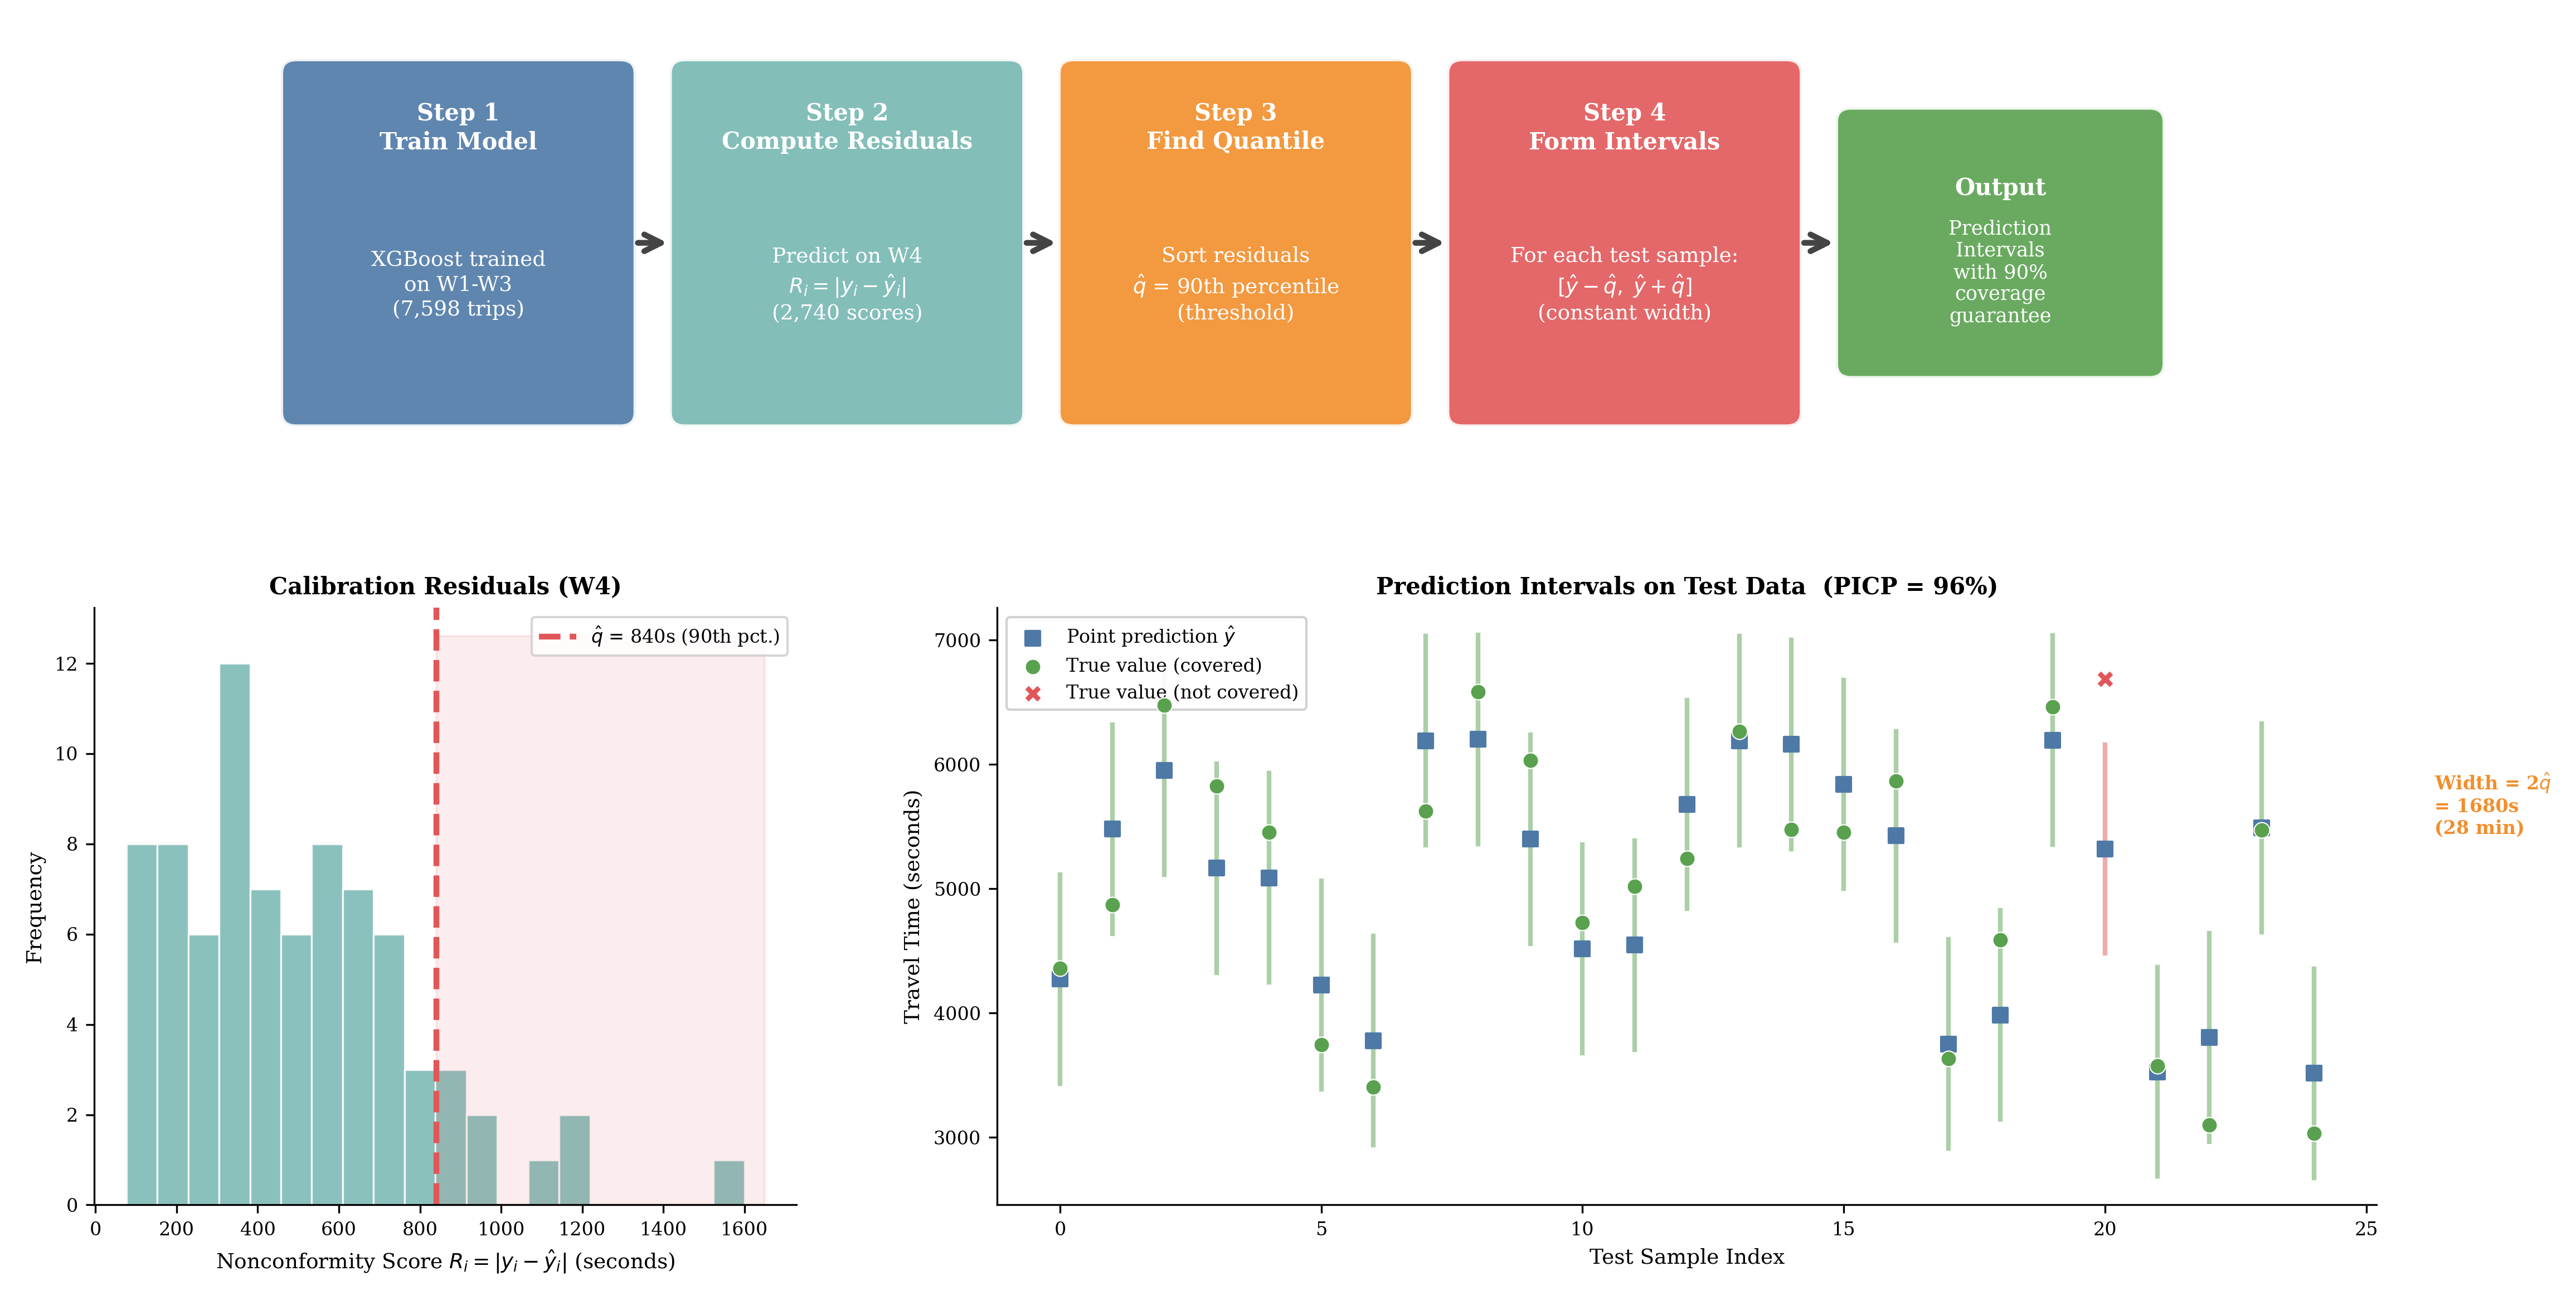
\includegraphics[width=\textwidth]{figures/3_5.png}
    \caption{Split conformal prediction process. The model is trained on W1--W3. Signed residuals are computed on the W4 calibration set. For a 90\% interval, the 5th and 95th percentiles of the shifted residual distribution define the lower and upper bounds around each test prediction.}
    \label{fig:cp_visualization}
\end{figure}

\subsubsection{Nonconformity Measure Variants}
\label{subsubsec:ncm_variants}

The baseline approach described above uses raw signed residuals to compute a single quantile from the entire calibration set. This is the absolute nonconformity measure. It treats all samples equally: every test point receives the same interval width regardless of its characteristics.

This thesis tests three additional NCM types that aim to improve interval efficiency by adapting the width to the sample context.

Mondrian: The calibration set is split into discrete bins based on categorical features. Each bin maintains its own residual distribution and quantile. A test sample receives an interval computed only from its bin's residuals. In this thesis, the bins are defined by time period (6 categories) crossed with route (3 routes), producing 15 active bins after merging a sparse night category into a global fallback. Mondrian CP is activated in \texttt{calibrated\_explanations} by passing a \texttt{bins} array to \texttt{calibrate()} and \texttt{explain\_factual()}.

Normalised with Difficulty Estimator (DE) : Instead of discrete bins, each sample receives a continuous difficulty score $\sigma_i$ from a KNN-based \texttt{DifficultyEstimator} ($k=25$). Calibration residuals are divided by their difficulty scores to produce normalised residuals, from which a single normalised quantile $\hat{q}_{\text{norm}}$ is computed. At prediction time, the interval is scaled by the test sample's difficulty: $[\hat{y} - \hat{q}_{\text{norm}} \cdot \sigma,\; \hat{y} + \hat{q}_{\text{norm}} \cdot \sigma]$. Easy samples get narrow intervals, hard samples get wide intervals.

Mondrian + DE : Both binning and difficulty scaling are applied simultaneously. The library computes per-bin normalised quantiles. Each test sample's interval depends on both its bin membership and its individual difficulty score. This is the most granular configuration.

Table~\ref{tab:ncm_experiments} summarizes which NCM types are used in each experiment.

\begin{table}[H]
\centering
\caption{NCM types used per experiment.}
\label{tab:ncm_experiments}
\begin{tabular}{lcccc}
\toprule
& \textbf{Absolute} & \textbf{Mondrian} & \textbf{Norm.\ DE} & \textbf{Mondrian + DE} \\
\midrule
Experiment 1 (RQ1) & \checkmark & & & \\
Experiment 2 (RQ2) & \checkmark & \checkmark & \checkmark & \checkmark \\
Experiment 3 (RQ3) & & & \checkmark & \\
\bottomrule
\end{tabular}
\end{table}

% ------------------------------------------------------------
\subsection{Experiment 1: Static Conformal Prediction Under Drift (RQ1)}
\label{subsec:exp1_method}
% ------------------------------------------------------------

\emph{How does temporal distribution shift affect the empirical coverage and interval efficiency of conformal prediction for bus ETA?}

In this experiment, the route-level XGBoost model is calibrated once using W4 data (2,745 trips). The calibration set is never updated after that. Prediction intervals are generated for all test periods (W5 through W8) without any modification to the calibration.

The conformal prediction is done through the \texttt{WrapCalibratedExplainer} class from the \texttt{calibrated\_explanations} library. The steps are:

\begin{algorithm}[H]
\caption{Static Conformal Prediction via \texttt{calibrated\_explanations}}
\label{alg:static_cp}
\begin{algorithmic}[1]
\REQUIRE Trained model $f$, calibration set $(X_{\text{cal}}, y_{\text{cal}})$, test set $X_{\text{test}}$, significance level $\alpha = 0.10$
\ENSURE Prediction intervals $[\ell_j, u_j]$ for each test sample $j$
\STATE $\text{explainer} \leftarrow \texttt{WrapCalibratedExplainer}(f)$ \COMMENT{Wraps pre-trained model}
\STATE $\text{explainer}.\texttt{calibrate}(X_{\text{cal}}, y_{\text{cal}})$ \COMMENT{Computes signed residuals, builds CPS}
\FOR{each test sample $x_j \in X_{\text{test}}$}
    \STATE $[\ell_j, u_j] \leftarrow \text{explainer}.\texttt{explain\_factual}(x_j, \text{low}=\alpha/2, \text{high}=1-\alpha/2)$
\ENDFOR
\RETURN $\{[\ell_j, u_j]\}_{j=1}^{|X_{\text{test}}|}$
\end{algorithmic}
\end{algorithm}

All test samples receive intervals from the same calibration. As time passes and the traffic distribution shifts, these intervals may become too narrow or too wide. The experiment measures this by evaluating PICP, MPIW, calibration error, and Winkler Score separately for each test period (Near, Mid, Far).

To check whether the findings depend on the chosen confidence level, the analysis is repeated at 80\% and 95\% in addition to the primary 90\% level.

% ------------------------------------------------------------
\subsection{Experiment 2: Online Adaptive Conformal Prediction (RQ2)}
\label{subsec:exp2_method}
% ------------------------------------------------------------

\emph{To what extent do online conformal methods improve empirical coverage stability and interval efficiency compared to static conformal approaches under drift?}

Online conformal prediction keeps the calibration set fresh. After predicting a batch of test samples and observing their true values, those samples are added to the calibration set before the next batch. The model itself is never retrained, only the calibration data changes.

\begin{algorithm}[H]
\caption{Online Conformal Prediction (Predict-then-Update)}
\label{alg:online_cp}
\begin{algorithmic}[1]
\REQUIRE Trained model $f$, initial calibration set $\mathcal{C}_0 = (X_{\text{cal}}, y_{\text{cal}})$, daily test batches $\{B_1, B_2, \ldots, B_D\}$, significance level $\alpha = 0.10$
\ENSURE Prediction intervals for all test samples
\STATE $\text{explainer} \leftarrow \texttt{WrapCalibratedExplainer}(f)$ \COMMENT{Wraps pre-trained model}
\FOR{each day $d = 1, \ldots, D$}
    \STATE $\text{explainer}.\texttt{calibrate}(\mathcal{C}_{d-1})$ \COMMENT{Optional: bins, difficulty\_estimator}
    \FOR{each sample $x_j \in B_d$}
        \STATE $[\ell_j, u_j] \leftarrow \text{explainer}.\texttt{explain\_factual}(x_j, \text{low}=\alpha/2, \text{high}=1-\alpha/2)$
    \ENDFOR
    \STATE Observe true values $\{y_j\}$ for $B_d$
    \STATE $\mathcal{C}_d \leftarrow \texttt{UpdateWindow}(\mathcal{C}_{d-1}, B_d)$ \COMMENT{Expanding or sliding window}
\ENDFOR
\end{algorithmic}
\end{algorithm}

The prediction happens \emph{before} the update. This is the standard predict-then-update protocol for online conformal prediction. It avoids using future information, the day's samples are only added to calibration after they have already been predicted.

\subsubsection{Window Strategies}

Three strategies for managing the calibration set were tested:

Expanding window: Every new batch is appended and nothing is removed. The calibration set starts at 2,745 samples (W4) and grows to about 12,066 by the end of the test period. This gives the most data for quantile estimation, but older data may not represent current conditions.

Sliding window (7-day): The calibration set is kept at a fixed size of 7 days samples. When new samples are added, the oldest are dropped. This keeps the calibration recent, but the smaller set means more noise in the quantile estimate.

Sliding window (14-day): A middle ground, about 14 days samples, balancing recency and stability.

\subsubsection{Factorial Design}

The four NCM types described in Section~\ref{subsubsec:ncm_variants} are combined with the four calibration strategies (Static, Online Expanding, Sliding-7d, Sliding-14d), producing a $4 \times 4$ factorial design of 16 configurations (Table~\ref{tab:factorial_design}). Algorithm~\ref{alg:online_cp} covers all 16: the \texttt{UpdateWindow} function selects the calibration strategy (column), while the optional \texttt{bins} and \texttt{difficulty\_estimator} parameters passed to \texttt{calibrate()} select the NCM type (row). Static CP is the special case where \texttt{UpdateWindow} returns the original calibration set unchanged.

\begin{table}[H]
\centering
\caption{The $4 \times 4$ factorial design: calibration strategy $\times$ NCM type.}
\label{tab:factorial_design}
\begin{tabular}{lcccc}
\toprule
& \textbf{Static} & \textbf{Online Exp.} & \textbf{Slide-7d} & \textbf{Slide-14d} \\
\midrule
Absolute & \checkmark & \checkmark & \checkmark & \checkmark \\
Mondrian & \checkmark & \checkmark & \checkmark & \checkmark \\
Normalised DE & \checkmark & \checkmark & \checkmark & \checkmark \\
Mondrian + DE & \checkmark & \checkmark & \checkmark & \checkmark \\
\bottomrule
\end{tabular}
\end{table}

% ------------------------------------------------------------
\subsection{Experiment 3: Segment-Level Uncertainty Decomposition (RQ3)}
\label{subsec:exp3_method}
% ------------------------------------------------------------

\emph{Can segment-level decomposition improve interval efficiency and support interpretable uncertainty attribution, and what is the resulting effect on empirical coverage?}

Experiments~1 and~2 work at the route level: the model predicts total trip time and the interval covers that total. A route-level interval tells the passenger how long the trip might take, but it does not say where the uncertainty comes from. A transit operator who wants to reduce travel time variability needs to know which segments of the route are the most unpredictable. Route-level CP also has no mechanism to exploit the internal structure of a trip for tighter intervals.

This experiment takes a different approach by changing the prediction granularity while keeping the same pre-departure setting as Experiments~1 and~2. The segment-level XGBoost model predicts every segment of the planned route at the moment of departure using only pre-trip features, and the per-segment predictions are combined back to the route level. This design targets two goals. First, segment-level prediction errors may partially cancel during summation, producing tighter route-level residuals and narrower intervals than a direct route-level prediction. Second, the per-segment difficulty scores enable uncertainty attribution, identifying which segments contribute most to route-level uncertainty.

\textbf{Why this experiment departs from the CPS approach.} Experiments~1 and~2 produce intervals through the \texttt{calibrated\_explanations} library, which wraps the Conformal Predictive System (CPS) directly around the XGBoost model output. The CPS pipeline requires that the conformal calibration step operates on the same objects the model was trained to predict. In Experiment~3, the conformal quantile is computed not on individual segment predictions but on route-level residuals obtained by summing segment predictions. Routing this aggregation step through the library pipeline would require bypassing several internal abstractions that are not designed for post-summation calibration. The manual split conformal procedure in Algorithm~\ref{alg:route_recal} is equivalent in principle --- it computes a quantile over held-out calibration residuals and applies it at prediction time --- but is implemented directly, prioritising transparency in demonstrating the residual-diversification mechanism. Specifically, the conformal quantile is computed as the $(1-\alpha)$-th percentile of the calibration residuals using \texttt{numpy.percentile} without a finite-sample correction factor. For the calibration sizes used here (350--700 trips per route-direction group), this difference from the corrected formula $\frac{\lceil(n+1)(1-\alpha)\rceil}{n}$ is negligible.

\subsubsection{Route-Level Re-Calibration}

The segment model is used for point predictions, but the prediction interval is calibrated at the route level. Summing segment-level intervals directly (lower bounds with lower bounds, upper bounds with upper bounds) would assume every segment simultaneously hits its extreme, producing near-perfect coverage but intervals too wide to be useful. Instead, the segment predictions are summed into a single route-level estimate, and a conformal quantile is computed from the route-level residuals.

A KNN-based \texttt{DifficultyEstimator} ($k=25$, scaled to $[0,1]$) is fitted on the calibration segments to assign each segment a difficulty score $\sigma_s$. This score is used in two ways: for the normalised re-calibration variant and for uncertainty attribution.

Algorithm~\ref{alg:route_recal} describes the absolute variant of the re-calibration procedure.

\begin{algorithm}[H]
\caption{Route-Level Re-Calibration from Segment Predictions}
\label{alg:route_recal}
\begin{algorithmic}[1]
\REQUIRE Trained segment model $f_s$, calibration trips $\{(X_s^{(i)}, T_{\text{actual}}^{(i)})\}_{i=1}^{N}$, significance level $\alpha = 0.10$
\ENSURE Route-level prediction intervals for test trips
\STATE \textbf{--- Calibration phase (once, on W4) ---}
\FOR{each calibration trip $i = 1, \ldots, N$}
    \STATE Predict every segment: $\hat{y}_s^{(i)} \leftarrow f_s(X_s^{(i)})$ for all segments $s$
    \STATE Sum to route level: $\hat{T}_{\text{route}}^{(i)} \leftarrow \sum_s \hat{y}_s^{(i)}$
    \STATE Compute residual: $R_i \leftarrow |T_{\text{actual}}^{(i)} - \hat{T}_{\text{route}}^{(i)}|$
\ENDFOR
\STATE Compute conformal quantile: $\hat{q}_{\text{route}} \leftarrow \text{Percentile}(\{R_i\}, 100(1-\alpha))$
\STATE
\STATE \textbf{--- Prediction phase (for each test trip) ---}
\FOR{each test trip $j$}
    \STATE Predict every segment: $\hat{y}_s^{(j)} \leftarrow f_s(X_s^{(j)})$ for all segments $s$
    \STATE Sum to route level: $\hat{T}_{\text{route}}^{(j)} \leftarrow \sum_s \hat{y}_s^{(j)}$
    \STATE Form interval: $[\hat{T}_{\text{route}}^{(j)} - \hat{q}_{\text{route}},\; \hat{T}_{\text{route}}^{(j)} + \hat{q}_{\text{route}}]$
\ENDFOR
\end{algorithmic}
\end{algorithm}

This re-calibration is done separately for each route $\times$ direction combination (6 groups, each with 350--700 calibration trips). Different routes have different lengths, segment counts, and traffic patterns. A single global quantile would average over these differences, producing intervals that are too wide for short routes and too narrow for long ones.

The key expectation behind this design is that segment-level prediction errors are not perfectly correlated across segments within a trip. When the model overpredicts one segment and underpredicts another, the errors partially cancel in the sum. This residual diversification should produce a tighter route-level residual distribution than the route model generates directly, leading to a smaller conformal quantile and narrower intervals.

\subsubsection{Normalised Variant}

A normalised variant adapts the interval width to the difficulty of each trip. Per-trip difficulty is computed as the sum of segment-level sigma values: $\sigma_{\text{trip}} = \sum_s \sigma_s$. During calibration, route-level residuals are divided by $\sigma_{\text{trip}}$ before computing the quantile, producing a normalised quantile $\hat{q}_{\text{norm}}$. At prediction time, the interval is scaled by the test trip's $\sigma_{\text{trip}}$:
\begin{equation}
    [\hat{T}_{\text{route}} - \hat{q}_{\text{norm}} \cdot \sigma_{\text{trip}},\; \hat{T}_{\text{route}} + \hat{q}_{\text{norm}} \cdot \sigma_{\text{trip}}]
\end{equation}

Trips composed of difficult segments get wider intervals. Trips composed of stable segments get narrower intervals. The total coverage is still controlled by the single quantile $\hat{q}_{\text{norm}}$, but the width is distributed according to each trip's difficulty composition.

\subsubsection{Uncertainty Attribution}

The difficulty scores from the \texttt{DifficultyEstimator} also enable uncertainty attribution. For each trip, the fraction of route-level uncertainty attributed to segment $s$ is:
\begin{equation}
    f_s = \frac{\sigma_s}{\sum_{s'=1}^{N} \sigma_{s'}}
    \label{eq:attribution}
\end{equation}

This fraction tells us what share of the total trip uncertainty comes from each segment. Values are between 0 and 1, and they sum to 1 across all segments in a trip. By averaging $f_s$ across all test trips, we identify structural uncertainty hotspots, segments that consistently contribute the most to route-level uncertainty regardless of the specific trip. This attribution comes from the difficulty estimator, not from the interval computation, so it is independent of whether the absolute or normalised re-calibration variant is used.


% ============================================================
\section{Reproducibility Details}
\label{sec:reproducibility}
% ============================================================

The full experimental pipeline is available online (to be published upon submission).\footnote{\url{https://github.com/kabuli-web/bus-eta-uncertainty}} All results in this thesis can be reproduced by running the notebooks in order, as described in the repository README.

\paragraph{Environment.} Python~3.10.0, run on AMD Ryzen 7~7435HS (8 cores, 3.1~GHz), 16~GB RAM. No GPU was used; all XGBoost training ran on CPU.

\paragraph{Key library versions.} \texttt{xgboost}~3.2.0, \texttt{scikit-learn}~1.7.2,\newline \texttt{calibrated-explanations}~0.11.0, \texttt{crepes}~0.9.0, \texttt{numpy}~2.2.6, \texttt{pandas}~2.3.3.

\paragraph{XGBoost hyperparameters.}
Table~\ref{tab:hyperparams_repro} lists the final hyperparameters for both models.
Hyperparameter search used randomised search with 50 configurations and temporal forward-chaining cross-validation, as described in Section~\ref{subsec:baseline_model}.

\begin{table}[H]
\centering
\caption{XGBoost hyperparameters for the route-level and segment-level models.}
\label{tab:hyperparams_repro}
\begin{tabular}{lcc}
\toprule
\textbf{Hyperparameter} & \textbf{Route-level} & \textbf{Segment-level} \\
\midrule
\texttt{n\_estimators}     & 500  & 200  \\
\texttt{max\_depth}        & 6    & 8    \\
\texttt{learning\_rate}    & 0.01 & 0.05 \\
\texttt{subsample}         & 0.9  & 0.9  \\
\texttt{colsample\_bytree} & 0.9  & 0.8  \\
\texttt{min\_child\_weight}& 3    & 3    \\
\texttt{reg\_lambda}       & 5    & 5    \\
\texttt{reg\_alpha}        & 0    & 0    \\
\bottomrule
\end{tabular}
\end{table}

\paragraph{Random seeds.} All random operations use seed~42: model training (\texttt{random\_state=42}), hyperparameter search (\texttt{random\_state=42}), and \texttt{DifficultyEstimator} $k$-NN fitting (\texttt{scaler=True}, \texttt{k=25}).

\paragraph{Dataset.} Mansurova et al.~\cite{mansurova2025dataset}. The processed parquet files used for all experiments are included in the repository.

% ============================================================
\section{Evaluation Metrics}
\label{sec:evaluation_metrics}
% ============================================================

Three point prediction metrics are used: Mean Absolute Error (MAE), Root Mean Squared Error (RMSE), and Mean Absolute Percentage Error (MAPE). MAE is the primary metric because it is interpretable in seconds and robust to the skewed error distributions in this data.

Four metrics evaluate prediction interval quality. Prediction Interval Coverage Probability (PICP) is the fraction of test samples where the true value falls inside the interval. A well-calibrated method at the 90\% level should have PICP close to 0.90. Mean Prediction Interval Width (MPIW) is the average width in seconds. Narrower intervals are preferred, provided coverage is adequate. Calibration Error is the absolute difference between empirical and nominal coverage: $|\text{PICP} - (1-\alpha)|$. Winkler Score combines width and coverage into a single metric. When the true value falls inside the interval, the score equals the width. When it falls outside, a penalty proportional to the miss distance is added, scaled by $2/\alpha$. Lower Winkler indicates better overall interval quality.


% ============================================================
% CHAPTER 4 — RESULTS
% ============================================================

\chapter{Results}
\label{ch:results}



% ============================================================
\section{Baseline Model Results}
\label{sec:baseline_results}
% ============================================================

Before reporting the conformal prediction experiments, we need to establish three properties of the baseline XGBoost models. First, whether point prediction accuracy drifts over time. Second, what the residuals look like. Third, whether segment-level difficulty varies across the route. These three properties directly shape the interpretation of every conformal prediction result that follows.

\subsection{Route-Level Model Performance}

Table~\ref{tab:route_performance} shows the route-level XGBoost performance across temporal periods.

\begin{table}[H]
\centering
\caption{Route-level XGBoost performance across temporal periods.}
\label{tab:route_performance}
\begin{tabular}{lrrrr}
\toprule
\textbf{Period} & \textbf{MAE (s)} & \textbf{RMSE (s)} & \textbf{MAPE (\%)} & \textbf{Samples} \\
\midrule
Calibration (W4) & 785.50 & 1,145.94 & 13.71 & 2,745 \\
Test-Near (W5) & 992.77 & 1,979.07 & 17.45 & 2,726 \\
Test-Mid (W6) & 859.42 & 1,234.93 & 15.95 & 1,844 \\
Test-Far (W7--W8) & 886.95 & 1,272.18 & 15.29 & 4,751 \\
\bottomrule
\end{tabular}
\end{table}

Test-period MAE ranges from 859~s (Test-Mid) to 993~s (Test-Near), against a calibration MAE of 786~s. Test-Far sits at 887~s, indicating that prediction error is consistently higher on test data than on calibration but does not increase monotonically with temporal distance: Test-Near contains the largest residuals, suggesting that day-to-day traffic variability dominates the error signal at this horizon. The RMSE values follow a similar pattern, with the largest gap between MAE and RMSE in Test-Near (993~s vs.\ 1979~s) pointing to a small number of trips with very large errors driving the average up.

% The RMSE-to-MAE ratio is about 1.4--1.5 across test periods. This gap between the two metrics is driven by a small number of trips with very large errors. It is the first sign that the residuals have heavy tails.


\subsection{Segment-Level Performance}

Table~\ref{tab:segment_performance} shows the segment-level model performance.

\begin{table}[H]
\centering
\caption{Segment-level XGBoost performance across temporal periods.}
\label{tab:segment_performance}
\begin{tabular}{lrrrr}
\toprule
\textbf{Period} & \textbf{MAE (s)} & \textbf{RMSE (s)} & \textbf{MAPE (\%)} & \textbf{Samples} \\
\midrule
% Train (W1--W3) & 44.91 & 105.68 & 95.14 & 302,609 \\
Calibration (W4) & 49.07 & 118.72 & 101.86 & 109,308 \\
Test-Near (W5) & 49.06 & 168.38 & 105.03 & 108,358 \\
Test-Mid (W6) & 49.19 & 120.70 & 116.73 & 73,161 \\
Test-Far (W7--W8) & 49.56 & 126.34 & 119.16 & 189,283 \\
\bottomrule
\end{tabular}
\end{table}

Segment MAE is essentially flat across the test period, ranging from 49.06~s in Test-Near to 49.56~s in Test-Far against a calibration MAE of 49.07~s. The MAPE values are high (around 100--120\%) because many segments have short run times (tens of seconds), where even a small absolute error becomes a large percentage. MAE is therefore the primary metric for segments.

The RMSE-to-MAE ratio sits between 2.4$\times$ and 3.4$\times$ at the segment level, much higher than the 1.4--2.0$\times$ at the route level. This means a small number of segments are much harder to predict than the rest. This spatial heterogeneity is what motivates Experiment~3: if all segments were equally difficult, decomposing the route into segments would add no information.


% ============================================================
\section{Experiment 1: Static Conformal Prediction Under Drift (RQ1)}
\label{sec:exp1_results}
% ============================================================

Static conformal prediction was applied to the route-level model with calibration done once on W4 and never updated.

\subsection{Overall Performance}

Table~\ref{tab:exp1_overall} shows the static CP results at the 90\% target coverage level across all test data combined (9,321 trips from W5--W8).

\begin{table}[H]
\centering
\caption{Static CP overall performance at 90\% target coverage, evaluated on the combined test set (W5--W8, 9,321 trips) and the W4 calibration set.}
\label{tab:exp1_overall}
\begin{tabular}{lrrrr}
\toprule
\textbf{Set} & \textbf{PICP} & \textbf{MPIW (s)} & \textbf{Cal.\ Error} & \textbf{Winkler} \\
\midrule
% Calibration (W4) & 0.9009 & 3,962 & 0.0009 & 5,439 \\
Test (W5--W8) & 0.8745 & 3,962 & 0.0255 & 6,449 \\
\bottomrule
\end{tabular}
\end{table}

On the test set, static CP achieves PICP of 0.8745, with a calibration error of 0.0255. The MPIW is 3,962 seconds (about 66 minutes) for trips that typically take 80--90 minutes. The interval is wide enough to absorb most of the temporal drift between calibration and test, but the resulting width consumes most of the trip duration itself \cite{Barber2023816}.

\subsection{Coverage by Test Period}

Table~\ref{tab:exp1_period} breaks down the test results by temporal period.

\begin{table}[H]
\centering
\caption{Static CP performance by test period (90\% target), evaluated separately on W4 (calibration), W5 (Test-Near), W6 (Test-Mid), and W7--W8 (Test-Far).}
\label{tab:exp1_period}
\begin{tabular}{lrrrrr}
\toprule
\textbf{Period} & \textbf{PICP} & \textbf{MPIW (s)} & \textbf{Cal.\ Error} & \textbf{Winkler} & \textbf{Trips} \\
\midrule
Test-Near (W5) & 0.8709 & 3,962 & 0.0291 & 7,900 & 2,726 \\
Test-Mid (W6) & 0.8693 & 3,962 & 0.0307 & 5,876 & 1,844 \\
Test-Far (W7--W8) & 0.8786 & 3,962 & 0.0214 & 5,839 & 4,751 \\
\bottomrule
\end{tabular}
\end{table}

At the 90\% level, per-period coverage falls from 0.9009 on the calibration set to 0.8709 on Test-Near, 0.8693 on Test-Mid, and 0.8786 on Test-Far. Calibration error sits between 0.021 and 0.031 across the test periods, against 0.0009 on calibration. The Winkler Score is highest on Test-Near (7,900), driven by the same heavy-tailed residuals that elevated the point-prediction RMSE in Section~\ref{sec:baseline_results}, and falls back to around 5,800--5,900 on Test-Mid and Test-Far. The MPIW is 3,962 seconds in every row because static CP fixes the interval width at calibration time and never adjusts it.

To test whether the small coverage drop is an artifact of wide intervals masking the drift, the analysis was repeated at 80\% and 95\% confidence levels. Table~\ref{tab:exp1_multiconf} shows the results.

\begin{table}[H]
\centering
\caption{Static CP coverage across confidence levels, evaluated on Test-Far (W7--W8, 4,751 trips): narrower intervals reveal larger drift effects.}
\label{tab:exp1_multiconf}
\begin{tabular}{lrrrrr}
\toprule
\textbf{Confidence} & \textbf{MPIW (s)} & \textbf{Cal.\ PICP} & \textbf{Far PICP} & \textbf{Drop (pp)} \\
\midrule
80\% & 2,660 & 0.7996 & 0.7615 & 3.8 \\
90\% & 3,937 & 0.8995 & 0.8771 & 2.2 \\
95\% & 5,074 & 0.9497 & 0.9364 & 1.3 \\
\bottomrule
\end{tabular}
\end{table}

As the confidence level decreases and the intervals become narrower, the coverage drop from calibration to Test-Far increases. At 80\%, where the interval width is 2,660 seconds (44 minutes) instead of 3,937 seconds (66 minutes), the drop reaches 3.8 percentage points. At 95\%, where the intervals are 5,074 seconds (85 minutes), the drop is only 1.3 percentage points.

These results are consistent with distribution shift affecting empirical coverage~\cite{Barber2023816}. The effect is modulated by interval width: narrower intervals show larger coverage drops than wider ones under the same shift, because a smaller interval has less margin to absorb the residual-distribution change between calibration and test.

Figure~\ref{fig:conditional_coverage} breaks down empirical coverage by time-of-day period and route, showing that the marginal PICP of 0.875 conceals substantial heterogeneity. Midday trips (09:00--16:00) consistently fall furthest below the 0.90 target, while evening trips (19:00--22:00) sit close to or above it. Route~12 shows systematically lower coverage than Routes~10 and~46 across all test periods. Night-time trips (22:00--05:00) had only 20 calibration samples in W4, indicating that the global fallback quantile is used for that stratum and its coverage estimate is unreliable. These subgroup patterns are consistent with temporal drift disproportionately affecting operating conditions whose travel-time distributions differ most from the calibration period.

\begin{figure}[H]
    \centering
    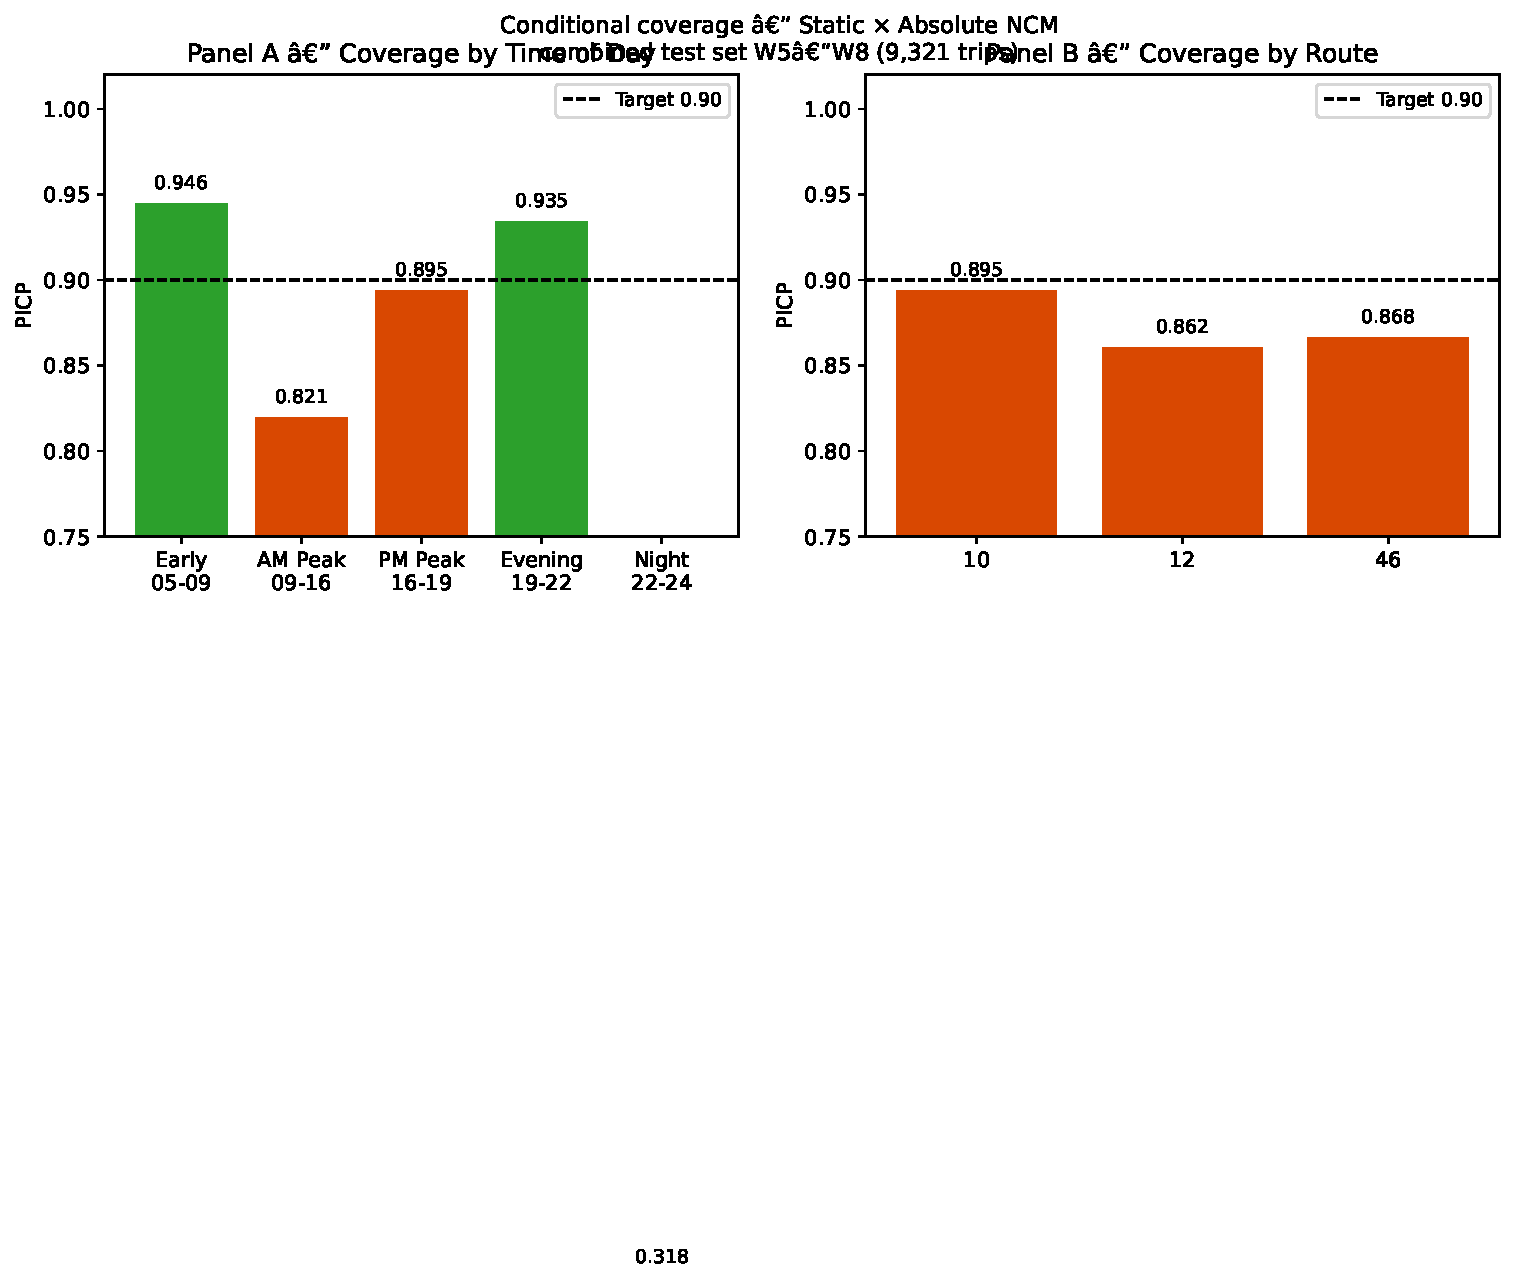
\includegraphics[width=\textwidth]{figures/exp1_conditional_coverage.pdf}
    \caption{Conditional coverage (PICP) of static CP broken down by time-of-day period (Panel A) and route (Panel B), evaluated on the combined test set W5--W8 (9,321 trips). The nominal target is 0.90 (dashed line). Night-time rows are excluded from Panel A due to insufficient calibration samples ($n \leq 20$). MPIW is identical across all subgroups (3,962 s) because static CP applies a single global quantile.}
    \label{fig:conditional_coverage}
\end{figure}

% ============================================================
\section{Experiment 2: Online Adaptive Conformal Prediction (RQ2)}
\label{sec:exp2_results}
% ============================================================


\subsection{Online CP vs Static CP}

Table~\ref{tab:exp2_online_vs_static} compares the three online window strategies against the static baseline, all using the standard absolute NCM.

\begin{table}[H]
\centering
\caption{Online CP vs Static CP at 90\% target (Absolute NCM), evaluated on the combined test set W5--W8 (9,321 trips)}
\label{tab:exp2_online_vs_static}
\begin{tabular}{lrrrr}
\toprule
\textbf{Method} & \textbf{PICP} & \textbf{MPIW (s)} & \textbf{Cal.\ Error} & \textbf{Winkler} \\
\midrule
Static & 0.8745 & 3,962 & 0.0255 & 6,449 \\
Online Expanding & 0.8901 & 4,207 & 0.0099 & 6,411 \\
Online Sliding-7d & 0.8964 & 4,302 & 0.0036 & 6,423 \\
Online Sliding-14d & 0.8933 & 4,259 & 0.0067 & 6,415 \\
\bottomrule
\end{tabular}
\end{table}

PICP rises from 0.875 (Static) to 0.890--0.896 under the three online strategies, a 1.5--2.1 percentage-point gain that brings empirical coverage closer to the 0.90 target.

Online methods help most on calibration error. Static CP has a calibration error of 0.0255, while Sliding-7d reduces it to 0.0036, an 86\% reduction relative to the static baseline. Sliding-14d and Online Expanding sit between these extremes.

The Winkler Scores are nearly identical across all four methods (range 6,411--6,449). Online recalibration shows no meaningful change in Winkler Score compared to static CP in the Absolute NCM setting; the gains here come from coverage tracking rather than width.

\subsection{Coverage Over Time}

\begin{table}[H]
\centering
\caption{Per-period coverage: Static vs Online Expanding (Absolute NCM), evaluated separately on Test-Near (W5), Test-Mid (W6), and Test-Far (W7--W8).}
\label{tab:exp2_period}
\begin{tabular}{lrr}
\toprule
\textbf{Period} & \textbf{Static} & \textbf{Online Exp.} \\
\midrule
Test-Near (W5) & 0.8709 & 0.8837 \\
Test-Mid (W6) & 0.8693 & 0.8921 \\
Test-Far (W7--W8) & 0.8786 & 0.8948 \\
\bottomrule
\end{tabular}
\end{table}

Online Expanding produces consistently higher coverage than Static across all three test periods, by 1.3--2.3 percentage points. Static coverage is lowest in Test-Mid (0.8693) while Online Expanding sits at 0.8921 there, indicating that the online strategy adapts the calibration quantile fast enough to compensate for residual-distribution shifts within the test window. The gap widens slightly with temporal distance from calibration, consistent with the role of adaptive recalibration under drift~\cite{Zaffran202225834}.

\subsection{Alternative Nonconformity Measures}

Three alternative NCM types were also tested: Mondrian (per-bin calibration), Normalised with Difficulty Estimator (per-sample scaling), and their combination. Together with the standard Absolute NCM, these form a $4 \times 4$ matrix of 16 configurations.

Table~\ref{tab:exp2_picp_matrix} shows the PICP for all 16 combinations.

\begin{table}[H]
\centering
\caption{PICP matrix: calibration strategy $\times$ NCM type (90\% target), evaluated on the combined test set W5--W8 (9,321 trips).}
\label{tab:exp2_picp_matrix}
\begin{tabular}{lrrrr}
\toprule
& \textbf{Static} & \textbf{Online Exp.} & \textbf{Slide-7d} & \textbf{Slide-14d} \\
\midrule
Absolute & 0.8745 & 0.8901 & 0.8964 & 0.8933 \\
Mondrian & 0.8702 & 0.8892 & 0.8978 & 0.8904 \\
Normalised DE & 0.8587 & 0.8635 & 0.8660 & 0.8673 \\
Mondrian + DE & 0.8557 & 0.8639 & 0.8715 & 0.8695 \\
\bottomrule
\end{tabular}
\end{table}

Table~\ref{tab:exp2_winkler_matrix} shows the Winkler Score for the same 16 combinations.

\begin{table}[H]
\centering
\caption{Winkler Score matrix: calibration strategy $\times$ NCM type (lower is better), evaluated on the combined test set W5--W8 (9,321 trips).}
\label{tab:exp2_winkler_matrix}
\begin{tabular}{lrrrr}
\toprule
& \textbf{Static} & \textbf{Online Exp.} & \textbf{Slide-7d} & \textbf{Slide-14d} \\
\midrule
Absolute & 6,449 & 6,411 & 6,423 & 6,415 \\
Mondrian & 6,200 & 6,164 & 6,168 & 6,178 \\
Normalised DE & 5,707 & 5,632 & 5,664 & 5,601 \\
Mondrian + DE & 5,827 & 5,551 & 5,752 & 5,591 \\
\bottomrule
\end{tabular}
\end{table}

Reading across a row shows the effect of calibration strategy. PICP and Winkler Score vary modestly across the four columns: PICP rises by 1--2~percentage points from Static to Online Sliding-7d in every NCM family, while Winkler Score moves by under 5\%. Online recalibration reduces calibration error rather than interval width, consistent with adaptive-conformal results in the literature~\cite{Zaffran202225834}.

Reading down a column shows the effect of NCM type. Moving from Absolute to Mondrian reduces Winkler by 4\%, and from Absolute to Normalised DE or Mondrian + DE reduces it by 11--14\%, regardless of calibration strategy. This is the efficiency dimension: difficulty-based normalisation redistributes interval width so that easy trips receive narrower intervals and hard trips receive wider ones, narrowing the average without sacrificing the marginal coverage guarantee~\cite{Romano2019}.

PICP also drops slightly under more adaptive NCMs because the redistributed intervals occasionally miss samples that would have been covered by the uniform wide interval; the same trade-off is documented for CQR-style adaptive intervals~\cite{Romano2019}.

The best Winkler Score overall is 5,551, achieved by Online Expanding $\times$ Mondrian + DE. The best PICP is 0.8978, achieved by Online Sliding-7d $\times$ Mondrian.

\subsection{Statistical Significance}

To assess whether performance differences across the 16 configurations are statistically reliable, the autorank procedure~\cite{Herbold2020autorank} was applied to per-sample Winkler scores across all 16 configurations on the combined test set. Figure~\ref{fig:autorank_cd} shows the critical difference (CD) diagram.

\begin{figure}[H]
    \centering
    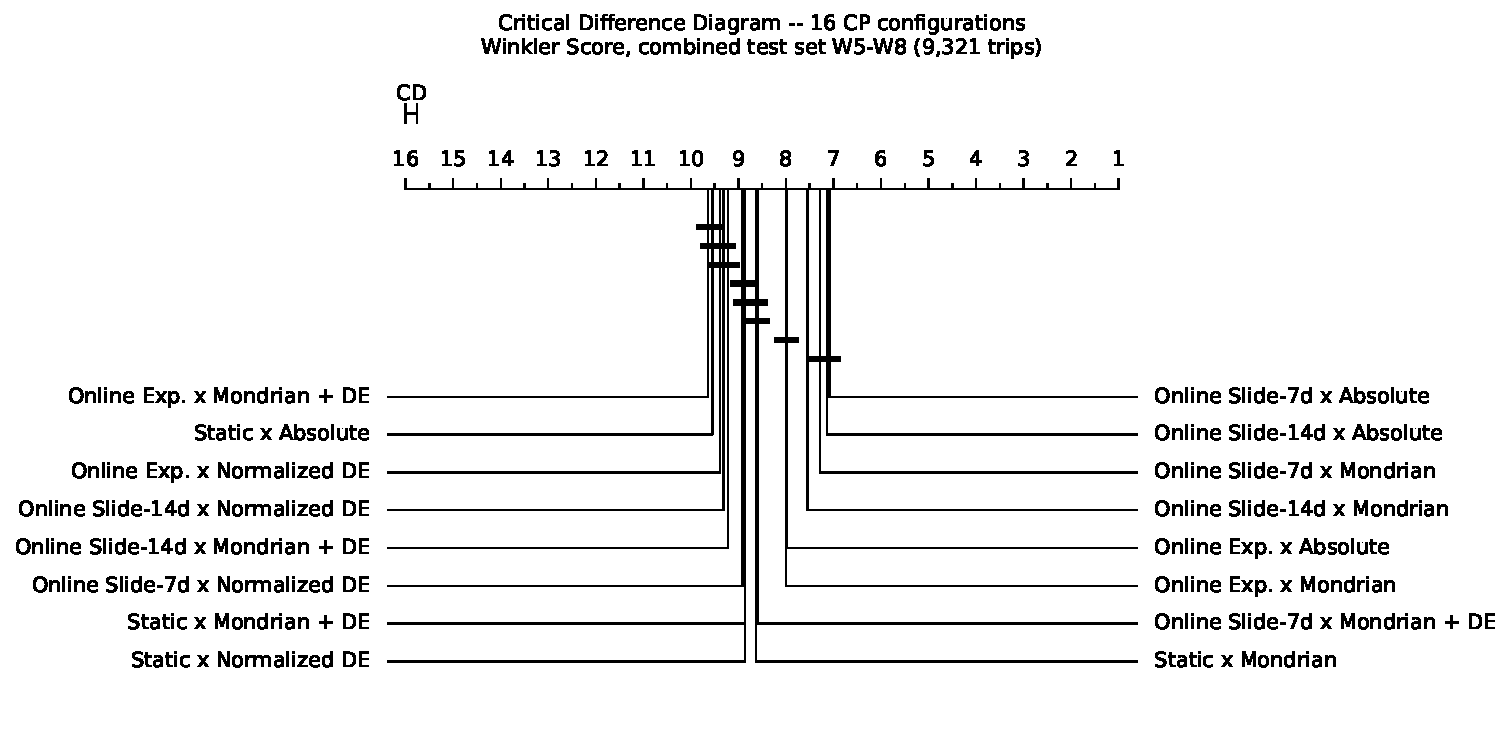
\includegraphics[width=\textwidth]{figures/autorank_cd.pdf}
    \caption{Critical difference diagram (autorank, $\alpha = 0.05$) comparing Winkler Score rankings across all 16 CP configurations on the combined test set W5--W8 (9,321 trips). Methods connected by a horizontal bar are not significantly different. Lower average rank = better Winkler Score performance.}
    \label{fig:autorank_cd}
\end{figure}

Per-sample Winkler scores for all 9,321 test trips were submitted to the autorank procedure, which applied Friedman's test (omnibus $p < 0.0001$) followed by Nemenyi post-hoc analysis at $\alpha = 0.05$. The mean Winkler scores separate clearly by NCM type: Mondrian~+~DE configurations achieve scores between 5,551 and 5,827, Normalised DE between 5,601 and 5,707, Mondrian between 6,164 and 6,200, and Absolute between 6,411 and 6,449. Within each NCM type the four calibration strategies differ by at most a few percent, compared to the 500--800~s gap between DE-based tiers and non-DE tiers. The critical difference diagram confirms that DE-based configurations are statistically superior to both Mondrian-only and Absolute configurations: the eight top-ranked configurations are all DE-based, the eight bottom-ranked are all non-DE. Effect sizes between configurations within the same NCM tier are small, confirming that the primary performance driver is NCM type rather than calibration strategy.


% ============================================================
\section{Experiment 3: Segment-Level Uncertainty Decomposition (RQ3)}
\label{sec:exp3_results}
% ============================================================


\subsection{Segment-Level Conformal Prediction}

The segment-level XGBoost model was calibrated with a KNN-based \texttt{DifficultyEstimator} on the W4 calibration segments. The difficulty estimator assigns each segment a continuous score reflecting how hard it is to predict, based on the residuals of its nearest neighbors in feature space. This score scales the interval width so that stable segments get narrow intervals and volatile segments get wide ones.

\subsection{Route-Level Re-Calibration}

The segment predictions are summed to produce a route-level point estimate, and a conformal quantile is computed at the route level. Table~\ref{tab:exp3_route_recal} compares several aggregation approaches against the direct route-level CP from Experiment~1.

\begin{table}[H]
\centering
\caption{Route-level comparison: Direct CP vs Segment Aggregation methods, evaluated on the combined test set W5--W8 (9,321 trips).}
\label{tab:exp3_route_recal}
\begin{tabular}{lrrrr}
\toprule
\textbf{Method} & \textbf{PICP} & \textbf{MPIW (s)} & \textbf{MPIW (min)} & \textbf{Winkler} \\
\midrule
Direct Route CP (Exp.~1) & 0.8745 & 3,962 & 66.0 & 6,449 \\
Re-Cal (Global) & 0.8790 & 2,502 & 41.7 & 4,287 \\
Re-Cal (Per-Route, Absolute) & 0.8882 & 2,323 & 38.7 & 4,035 \\
Re-Cal (Per-Route, Norm.\ DE) & 0.8882 & 2,323 & 38.7 & 4,035 \\
\bottomrule
\end{tabular}
\end{table}

Route-level re-calibration calibrates a single conformal quantile on summed segment predictions at the route level, rather than summing individual segment intervals. The improvement over direct route CP is substantial. MPIW drops from 3,962~s (66 minutes) to 2,323~s (39 minutes), a reduction of 41\%. The Winkler Score improves from 6,449 to 4,035, a 37\% improvement. Empirical coverage rises from 0.875 to 0.888, slightly above the 0.875 marginal level seen for direct route CP and just under the 0.90 nominal target.

The segment model produces narrower intervals through the residual diversification effect described in Section~\ref{subsec:exp3_method}: segment-level prediction errors partially cancel during summation, producing a tighter route-level residual distribution and a smaller conformal quantile. Variance-of-sums reasoning predicts this whenever per-segment residuals have low pairwise correlation~\cite{Romano2019}.

To verify the residual diversification mechanism, we analysed per-segment prediction residuals $r_s = y_s - \hat{y}_s$ across W4 calibration trips. All 2,745 calibration trips (100\%) contained both positive and negative segment-level residuals, confirming that no trip is uniformly over- or under-predicted across all segments. The mean lag-1 autocorrelation of segment residuals within a trip was close to zero, indicating that consecutive segment residuals are effectively uncorrelated. This near-independence means that errors do not systematically accumulate; instead, they partially cancel during summation. Empirically, the standard deviation of route-level residuals is 1,145~s for the direct route model and 796~s for the summed segment model, a 30.5\% reduction. This variance reduction is directly reflected in the 41\% MPIW improvement observed in Table~\ref{tab:exp3_route_recal}.

Figure~\ref{fig:segment_residuals} illustrates the diversification mechanism for a representative trip.

\begin{figure}[H]
    \centering
    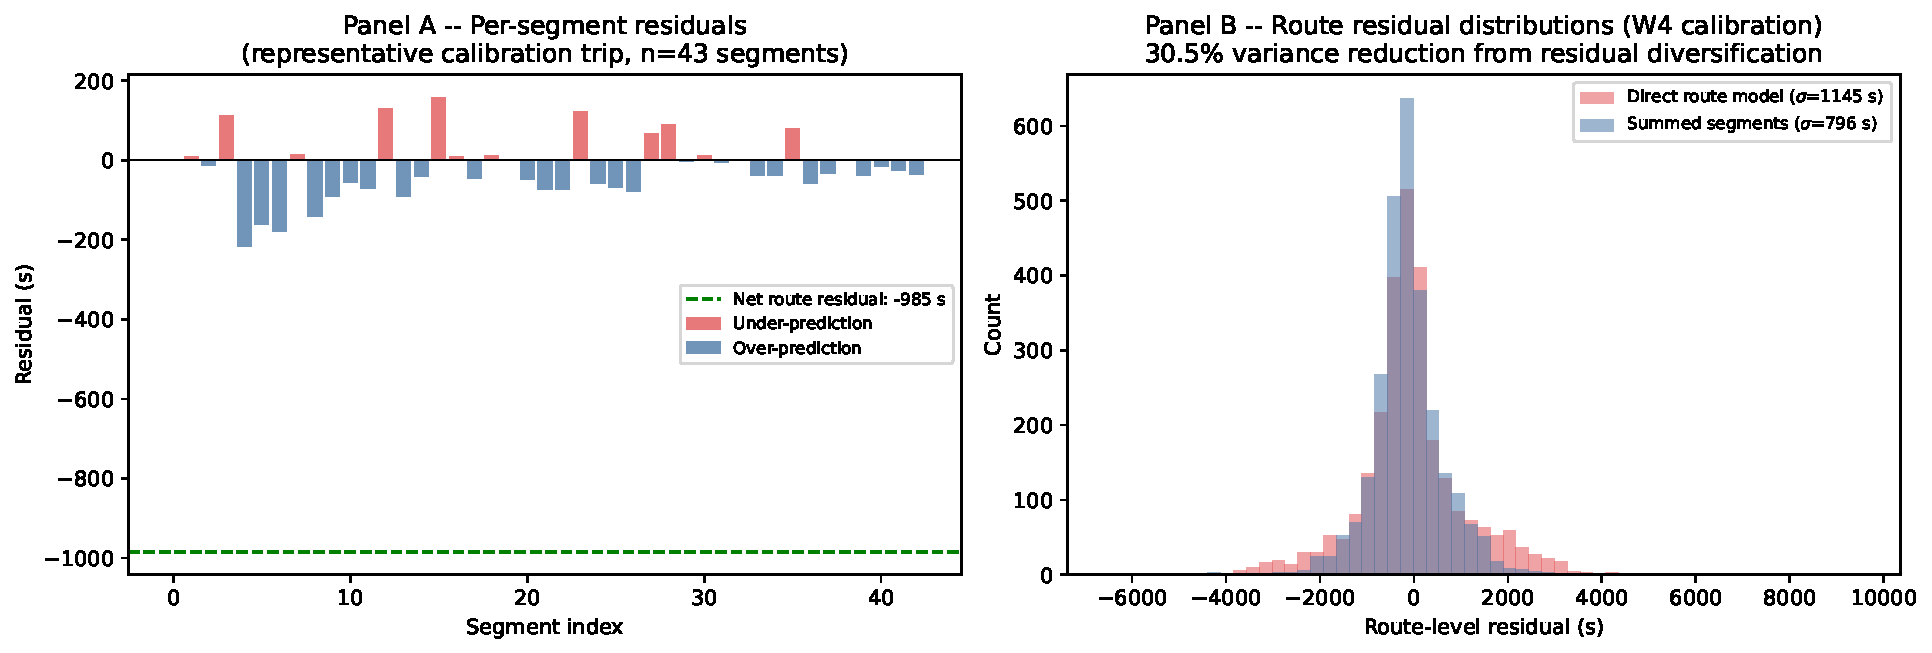
\includegraphics[width=\textwidth]{figures/exp3_residual_diversification.pdf}
    \caption{Residual diversification in segment-level predictions, computed on the W4 calibration set. \textit{Panel A:} per-segment signed residuals ($r_s = y_s - \hat{y}_s$) for a representative trip, with positive bars indicating under-prediction and negative bars indicating over-prediction. The dashed line shows the net route-level residual (close to zero), demonstrating near-perfect cancellation for this trip. \textit{Panel B:} distribution of route-level point-prediction residuals from the direct route model ($\sigma = 1{,}145$~s) and the summed segment model ($\sigma = 796$~s), confirming the variance reduction attributable to residual diversification.}
    \label{fig:segment_residuals}
\end{figure}

As described in Section~\ref{subsec:exp3_method}, the re-calibration is done per route and direction. The normalised variant produces the best Winkler Score by adapting the interval to each trip's difficulty composition.

\subsection{Uncertainty Attribution}

\begin{table}[H]
\centering
\caption{Top 5 segments by uncertainty attribution (sigma-based fraction), averaged across all test trips (W5--W8, 9,321 trips).}
\label{tab:exp3_attribution}
\begin{tabular}{rrrr}
\toprule
\textbf{Segment} & \textbf{Direction} & \textbf{Mean Width (s)} & \textbf{Fraction} \\
\midrule
1 & 0 & 1,826.8 & 23.34\% \\
17 & 1 & 284.3 & 4.24\% \\
15 & 1 & 233.9 & 3.46\% \\
21 & 1 & 219.0 & 3.46\% \\
18 & 0 & 249.3 & 3.30\% \\
\bottomrule
\end{tabular}
\end{table}

The attribution table is dominated by Segment~1 in Direction~0, which alone accounts for 23.34\% of the per-trip uncertainty budget --- almost an order of magnitude more than the next-largest contributor. Inspecting the raw segment travel-time distribution explains why: in Direction~0, Segment~1 has mean run time 916~s and standard deviation 1{,}033~s, against an overall segment mean of 105~s and standard deviation 188~s; the same segment position in Direction~1 has mean 63~s and standard deviation 101~s. The asymmetry between directions points to a structural property of the data rather than a traffic phenomenon: in Direction~0 the first recorded segment absorbs the origin-terminal dwell and the vehicle's pull-out interval, during which the actual start of the trip can lag the scheduled start by several minutes. The historical-statistic features (\texttt{hist\_seg\_mean}, \texttt{hist\_seg\_std}) reflect this elevated variance, the difficulty estimator inherits it, and the attribution procedure reports it as the dominant uncertainty source. The remaining four entries in the top five sit in the 3--5\% range and correspond to mid-route segments where local traffic patterns increase travel-time variability without changing the overall route-level interval. For an operator, this output separates measurement-process artefacts (Segment~1, Direction~0) from genuine spatial uncertainty hotspots (Segments 15--21), which is the kind of distinction that route-level CP cannot surface.


% ============================================================
% DISCUSSION AND LIMITATIONS
% ============================================================

\chapter{Discussion}
\label{ch:discussion}



% ============================================================
\section{Discussion of Findings}
\label{sec:discussion_findings}
% ============================================================

\subsection{Marginal Coverage as a Misleading Metric (RQ1)}

The central finding of Experiment~1 is that static CP maintains marginal coverage near the 90\% target despite statistically significant distribution shift. The coverage drop from calibration to Test-Far is consistent with findings in the broader conformal prediction literature, where moderate distribution shift under static calibration typically produces single-digit coverage losses. The multi-confidence analysis (Table~\ref{tab:exp1_multiconf}) reinforces this: the same shift produces larger coverage drops at lower confidence levels where intervals are narrower, confirming that drift is present at every level with its magnitude modulated by interval width.

The more important finding is that marginal coverage is a misleading quality indicator in this domain. Reporting only PICP at a single confidence level can obscure the real problem. As shown in Table~\ref{tab:exp1_overall}, the intervals are wide enough to cover most outcomes but too wide to be operationally useful for trips of this duration. The Winkler Score, which penalizes both missed predictions and excessive width, gives a more complete picture.

This reframes the practical challenge. The question is not whether CP maintains coverage under drift, it does to a degree. The question is whether the intervals are narrow enough to be informative. Bus travel time prediction inherently produces substantial residuals due to heterogeneous traffic conditions, variable dwell times, and route-specific dynamics. The resulting prediction intervals reflect this difficulty.

To answer RQ1: temporal distribution shift produces measurable but moderate coverage degradation. The dominant effect is on interval efficiency, not coverage.

This finding is consistent with Barber et al.~\cite{Barber2023816}, who showed that coverage guarantees weaken under covariate shift. The 2--3 percentage-point degradation observed here is mild relative to more severe drift scenarios, likely because the temporal gap between calibration and test spans only 1--4 weeks and the model's residual distribution changes gradually. Petelin et al.~\cite{Petelin2024} evaluated CP for traffic forecasting under approximately i.i.d.\ conditions; the present results extend that work by quantifying coverage degradation under measured temporal drift.

\subsection{Efficiency as the Primary Improvement Axis (RQ2)}

Since marginal coverage is already adequate, the main contribution of the factorial comparison (Tables~\ref{tab:exp2_picp_matrix} and~\ref{tab:exp2_winkler_matrix}) is on the efficiency dimension. NCM sophistication, particularly difficulty estimation, provides the dominant Winkler improvement. These gains come from redistributing the uncertainty budget: easy-to-predict trips get narrower intervals and hard-to-predict trips get wider ones, without changing the total coverage.

Online recalibration contributes primarily to calibration precision rather than coverage or efficiency. It reduces calibration error (Table~\ref{tab:exp2_online_vs_static}) but the Winkler Score barely changes because the overall interval width is dominated by the prediction difficulty of the task, not by the freshness of the calibration set. In domains where prediction models achieve lower residuals and narrower intervals, the relative contribution of online recalibration would likely increase.

The factorial design confirms that calibration strategy and NCM type operate on different aspects of interval quality and can be chosen independently. This is a practical finding for system design: an operator can select the calibration update frequency based on data availability and computational constraints, and separately choose the NCM based on the desired trade-off between average width and per-sample adaptation. However, even the best route-level configuration still produces intervals that are too wide for operational use.

To answer RQ2: online recalibration improves calibration precision but not interval efficiency. NCM sophistication is the effective lever at the route level. The route-level efficiency ceiling motivates the segment-level approach.

The efficiency gains from difficulty-based normalisation align with CQR~\cite{Romano2019}, which also adapts interval width to sample difficulty and has been shown to produce narrower intervals in heteroskedastic settings. The marginal benefit of online recalibration observed here is lower than in ACI-based frameworks~\cite{Zaffran202225834}, likely because the base model's residual variance is high: when prediction intervals are already wide, the recency of calibration samples contributes diminishing returns to overall interval quality.

\subsection{Segment Decomposition as an Efficiency Strategy (RQ3)}

Since route-level strategies reached their efficiency limit, Experiment~3 takes a different approach by changing the prediction granularity. As shown in Table~\ref{tab:exp3_route_recal}, segment-level decomposition with route-level re-calibration produces the largest efficiency improvement of any method tested, substantially outperforming both direct route CP and the best route-level NCM configuration.

This improvement is consistent with the hypothesis of residual diversification: segment-level errors partially cancel during summation, as described in Section~\ref{subsec:exp3_method} and reflected by the substantially narrower route-level residuals in Table~\ref{tab:exp3_route_recal}. Direct empirical evidence for this mechanism --- showing that positive and negative segment residuals coexist within individual trips --- is presented in Section~\ref{sec:exp3_results}.

The uncertainty attribution (Table~\ref{tab:exp3_attribution}) adds an interpretability layer that route-level CP cannot provide. The concentration of uncertainty in a small set of segments gives a transit operator a specific spatial target for intervention or further investigation. The persistence of these hotspots across test periods confirms that they reflect fixed properties of the route or its data-collection geometry rather than transient traffic conditions.

To answer RQ3: segment-level decomposition produces substantially narrower intervals than any route-level method and enables spatial uncertainty attribution while keeping empirical coverage close to the nominal target (0.888 against 0.90). The approach is best interpreted as a finer-grained pre-departure interval estimator that simultaneously improves efficiency and supports per-segment interpretability.

The efficiency gain from segment-level decomposition is consistent with findings in link-based prediction~\cite{Chen201160}, where finer spatial granularity reduces unexplained variance in route-level aggregations. The use of difficulty-based width scaling parallels normalised CP~\cite{Romano2019}, though applied here at the trip level (by summing segment difficulty scores) rather than at the individual sample level.

The practical utility of a prediction interval depends on the decision it supports. For a passenger deciding whether to run for a departing bus, a 39-minute uncertainty window for a 90-minute trip may narrow the decision space meaningfully. For a passenger deciding whether to leave home to catch a specific departure, a 15-minute window would be more actionable, and the current results do not reach that threshold. The framework does not specify a target interval width; what constitutes an operationally useful interval will differ by use case, route frequency, and passenger tolerance for missed connections. A 66-minute interval for a 90-minute trip, for example, spans nearly the entire plausible range of travel times and offers no useful guidance for any time-sensitive passenger decision. Operators considering deployment should define an interval-width threshold that corresponds to actionable passenger decisions for their specific service patterns, and use that threshold to evaluate whether the segment-level approach meets operational requirements.

% ============================================================
\section{Ethics and Societal Implications}
\label{sec:ethics}
% ============================================================

\subsection{Data Privacy and Governance}

The dataset used in this thesis is derived from GPS bus traces published by Mansurova et al.~\cite{mansurova2025dataset} as open GTFS data. Records are aggregated at the segment level and contain no personally identifiable passenger information. Nevertheless, GPS trajectory data from vehicles can in principle be linked to driver movement patterns. Responsible use of such data requires that no individual-level records be retained beyond what is necessary for the analysis, that the data be used only for the stated research purpose, and that any derivative outputs respect the terms of the original publication. These principles were followed throughout this study.

\subsection{Fairness and Service Equity}

Calibration quality in this framework is not uniform across all passenger groups. The night-period category (22:00--05:00) had only two calibration samples in W4, which was insufficient for the Mondrian binning approach and required a global fallback. As a result, night-time passengers receive wider, less adapted uncertainty estimates than passengers during peak or midday periods. Similarly, routes or directions with fewer trips will produce noisier calibration quantiles and potentially less reliable intervals. Deploying the framework uniformly across all time periods and routes without auditing per-subgroup calibration could mean that passengers who depend on low-frequency or night services --- often those with fewer transportation alternatives --- systematically receive worse uncertainty information without any indication that this is the case. Any operational deployment should include explicit monitoring of calibration quality per subgroup before release.

\subsection{Operational Consequences of Miscalibrated Intervals}

Under-covering intervals (too narrow relative to the nominal level) create overconfident uncertainty estimates. A passenger who trusts a narrow interval may act on it --- leaving home at a specific time, for instance --- and miss a bus when the true arrival falls outside the stated range. The broader societal consequence is a loss of trust in the ETA system that is difficult to recover once passengers have been burned by unreliable estimates.

Conversely, intervals that are too wide (as observed at the route level: 60+ minutes for a 90-minute trip) may be so uninformative as to be useless, leading passengers to ignore the uncertainty estimate entirely. The segment-level approach reduces this problem substantially (39-minute intervals at 0.888 empirical coverage), but operators should still communicate that the interval reflects a statistical property across many trips, not a promise for any individual journey, and that empirical coverage trails the nominal 90\% target by a small margin.

\subsection{Responsibility Under Temporal Drift}

The framework's empirical coverage degrades as time passes from calibration. In a deployed system, this means that an operator who sets up conformal calibration once and does not update it will gradually deliver worse uncertainty estimates to passengers. The responsibility for monitoring and recalibrating the system on a defined schedule rests with the transit operator. Automated uncertainty estimation systems should not be treated as set-and-forget infrastructure; they require the same operational oversight as the point prediction models they wrap.

\subsection{Sustainable Development}

More reliable ETA interval estimates have the potential to reduce unnecessary waiting at bus stops, improve trip planning, and reduce missed connections --- contributing to more efficient and attractive public transport. Greater transit ridership, in turn, can reduce private car use and associated carbon emissions. The computational overhead of the online recalibration approach evaluated in this thesis is low: calibration updates require only a percentile computation over a sliding window of recent residuals and can run in milliseconds. This makes the framework feasible for operational deployment without significant energy cost.

\subsection{Human-Centred Use}

Prediction intervals produced by conformal prediction are statistical objects. A 90\% prediction interval means that, across many similar trips, approximately 90\% of true travel times will fall within the stated range. It is not a guarantee for any individual trip. Any transit information system that presents these intervals to passengers must communicate this distinction clearly and avoid implying false precision. Interval estimates should support passenger and operator decision-making rather than replace it; operators should retain the ability to override or contextualise automated uncertainty outputs when local knowledge or real-time information suggests the statistical estimate may be unreliable.

% ============================================================
\section{Limitations}
\label{sec:limitations}
% ============================================================

\subsection{Single City and Limited Observation Period}

The dataset covers three bus routes in Astana, Kazakhstan, over 55 days from late July to late September 2024. Different cities may have different drift patterns depending on climate, infrastructure, and operational practices. The 55-day window captures one seasonal transition (summer to early autumn) but does not include winter conditions, holidays, or major infrastructure changes. The distribution shift observed over this period is moderate, producing 1--4~pp coverage drops depending on confidence level. Longer observation periods spanning multiple seasons would likely produce stronger drift and more pronounced effects on coverage. The findings are specific to this dataset and would need to be replicated in other settings to establish generalizability.

\subsection{Single Model Architecture}

Only XGBoost was used as the point prediction model. Deep learning models such as LSTM, GRU, or Transformer architectures may produce residuals with different statistical properties, which could affect the conformal prediction behaviour. The coverage degradation under drift is likely model-independent since it stems from distributional shift rather than model architecture. However, the specific coverage values and interval widths reported in this thesis may differ with other models.

\subsection{No Model Retraining}

The XGBoost model was trained once on W1--W3 and kept fixed throughout all experiments. Only the calibration set was updated in the online experiments. In a real deployment, periodic model retraining would improve point prediction accuracy and likely improve conformal prediction quality as well. The results in this thesis therefore represent a conservative scenario where only the calibration layer adapts while the underlying model stays frozen.

\subsection{No External Variables}

The dataset does not include weather data, special events, or real-time traffic information. These factors can cause sudden distribution shifts that are different from the gradual seasonal drift observed in this study. The framework's behaviour under abrupt, event-driven drift was not evaluated.

\subsection{Night Period Data Scarcity}

The night period (22:00--05:00) had only 2 calibration samples in W4. This was insufficient for Mondrian binning, and a global fallback was used instead. The framework cannot provide category-specific intervals for time periods with very sparse data. In a production system, longer data collection periods or pooling across routes could address this limitation.

% ============================================================
% CONCLUSION
% ============================================================

\chapter{Conclusion}
\label{ch:conclusion}


% ============================================================
\section{Contributions}
\label{sec:contributions}
% ============================================================

This thesis makes four contributions to the empirical study of uncertainty-aware bus ETA prediction, demonstrated on a real-world GTFS dataset from Astana, Kazakhstan.

First, it provides empirical evidence that marginal coverage alone is a misleading indicator of conformal prediction quality under temporal distribution shift on this dataset. A multi-confidence analysis shows that the same drift produces different coverage effects depending on interval width, and that the dominant practical impact is on interval efficiency rather than coverage. Joint assessment of coverage and efficiency dimensions is necessary to characterise CP behaviour under drift.

Second, it provides a factorial evaluation showing that calibration freshness and NCM sophistication are two largely independent dimensions of interval quality in this setting. Difficulty-based normalisation is the most effective route-level lever for improving interval efficiency, operating independently of the calibration update strategy.

Third, it provides empirical evidence that route-level re-calibration applied to summed segment-level predictions can substantially reduce interval width, consistent with residual diversification during summation. On this dataset, changing prediction granularity produces larger efficiency gains than optimising the nonconformity measure or calibration strategy within the route-level framework.

Fourth, it introduces sigma-based uncertainty attribution that quantifies each segment's contribution to route-level uncertainty on a per-trip basis, demonstrating that conformal prediction combined with difficulty estimation can localise uncertainty to specific spatial components of a route.


% ============================================================
\section{Future Work}
\label{sec:future_work}
% ============================================================

The findings and limitations of this thesis point to several directions for future research.

ACI \cite{Gibbs2024} is an online learning procedure that adjusts the target significance level based on recent coverage errors, providing long-run average coverage without requiring exchangeability. It is not a conformal method itself but a sequential wrapper that modifies the input to any interval construction procedure. In settings with better-trained models and narrower intervals, where drift would cause visible coverage loss, ACI would be a natural complement to the conformal framework evaluated here.

In this thesis, online recalibration (Experiment~2) and segment decomposition (Experiment~3) were tested separately to isolate their individual effects. Combining them, online updates to the segment-level calibration with route-level re-calibration, could deliver both temporal adaptation and spatial interpretability. This combination was not tested due to the experimental isolation design but represents the most complete version of the proposed framework.

The dataset covers three routes in one city over 55 days. Replicating the experiments on datasets with longer observation periods, covering multiple seasons and capturing stronger drift, would test whether the coverage-efficiency trade-off observed here changes under more severe distribution shift. The GTFS-based data format is a worldwide standard, making cross-city replication straightforward in terms of data structure.

Additional directions include exploring the effect of different model architectures (LSTM, Transformer) on conformal prediction behaviour and the integration of external variables (weather, events) to improve both point predictions and calibration under sudden shifts.

\bibliographystyle{IEEEtran}
\bibliography{references}

\end{document}